\section{Probability Distributions}\label{cha:probDecomposition}

In this chapter we will establish relations between the formalism of tensor networks and basic concepts of probability theory.
We will first understand distributions as tensors and connect their marginalizations and conditionings to the tensor operations of contractions and normations.
Then we discuss independence assumptions as examples of contraction equations, which lead to tensor network decompositions known as graphical models.
We then treat more generic exponential families and investigate their representation as tensor networks.

\subsection{Tensor Representation of Distributions}

%% Random Variables: Introduction in Bayesian way by uncertainties
After having discussed how to represent states of factored systems by one-hot encodings, let us now take advantage of these representation by associating properties with these states.
Let there be uncertainties of the assignments $\catindexof{\atomenumerator}$ to the categorical variables $\catvariableof{\atomenumerator}$ of a factored system.
We then understand $\catvariableof{\atomenumerator}$ as random variables, which have a joint distribution defined by the uncertainties of the state assignments.
To capture these uncertainties we now make use of the one-hot representation of factored systems in Chapter~\ref{cha:factoredRepresentation}.

\begin{definition}[Probability Tensor] % From the axioms of Kolmogorov!
	Let there be a factored system defined by a categorical variable $\catvariableof{\atomenumerator}$ for each $\atomenumeratorin$ taking values in $[\catdimof{\atomenumerator}]$. 
	A probability distribution over the states of $\facsystem$ is a tensor
		\[ \probat{\catvariableof{0},\ldots,\catvariableof{\atomorder-1}} : \facstates \rightarrow [0, 1] \subset \rr \]
	such that
		\[ \sum_{\catindices\in\facstates} \probat{\indexedcatvariables} = 1 \, . \]
\end{definition}

We notice that there are two conditions for a tensor to be probability tensor.
First, the tensor needs to have non-negative coordinates and second, the coordinates need to sum to $1$.

%% One-hot Decomposition -> Contraction Equivalences
The probability tensor to the distribution is an object
		\[ \probat{\catvariables} \in \bigotimes_{\atomenumeratorin}\rr^{\catdimof{\atomenumerator}} \]
which is the sum over the one-hot encodings (see Lemma~\ref{lem:tensorBasisDecomposition})
		\[ \probat{\catvariables} = \sum_{\catindices\in\facstates} \probat{\indexedcatvariables} \cdot \onehotmapofat{\catindices}{\catvariables} \, . \]
		
%%
The normation condition of probability tensors can be expressed by the contraction equation $1= \sbcontraction{\probtensor}$ since
\begin{align*}
	1 = \sum_{\catindices}\probat{\indexedcatvariables}
	=  \sum_{\catindices}\sbcontraction{\probtensor, \onehotmapof{\catindices}}
	= \sbcontraction{\probtensor} \, . 
\end{align*}

%% NOT NEEDED
%Using the Coordinate Calculus as described in Theorem~\ref{the:coordinateCalculus} we can retrieve the coordinates of $\probtensor$ storing the probabilities of specific states by the contraction
%\begin{align*}
%	\probat{\indexedcatvariables} = \contractionof{\{\probtensor, \onehotmapof{\catindices}\}}{\varnothing} \, . 
%\end{align*}

%% Coordinates
%The probability tensor stores all probabilities on its coordinates, which are by construction
%	\[ \probtensor_{\catindices} = \probat{\catvariableof{\atomenumerator} = \catindexof{\atomenumerator} \, : \, \atomenumeratorin}  \, . \]
%We here draw on the redundancy of the one-hot encoding of each state of a factored system, which enables us to represent the properties of multiple states in single tensors (see Example~\ref{exa:onehotUncertainty}).

Probability tensors are depicted as
\begin{center}
	


\begin{tikzpicture}[scale=0.35,thick] % , baseline = -3.5pt

\node[anchor=center] (text) at (-2,0) {$a)$};

\node [circle, draw, thick, fill=gray!50, minimum size = \nodeminsize] (P1) at (0,-3) {\tiny $\catvariableof{0}$};	
\node [circle, draw, thick, fill=gray!50, minimum size = \nodeminsize] (P2) at (3,-3) {\tiny $\catvariableof{1}$};

\node[anchor=center] (text) at (6,-3) {$\cdots$};

\node [circle, draw, thick, fill=gray!50, minimum size = \nodeminsize] (P3) at (9,-3) {};

\node[anchor=center] (text) at (9,-3) {\tiny $\catvariableof{\atomorder-1}$};


\draw[midarrow] 
    	(4.5,0) to[bend right=25] (P1);
\draw[midarrow] 
    	(4.5,0) to[bend right=10] (P2);
\draw[midarrow] 
	(4.5,0) to[bend right=-25] (P3);
	
\node[anchor=center] (text) at (4.5,0.5) {$\edge$};


\begin{scope}[shift={(20,0)}]

\node[anchor=center] (text) at (-2,0) {$b)$};

\draw (-1,-1) rectangle (5,-3);
\node[anchor=center] (text) at (2,-2) {\small $\probtensor$};
%\draw[->] (0,-3)--(0,-5) node[midway,left] {\tiny $\catlegof{0}$}; 
%\draw[->] (1.5,-3)--(1.5,-5) node[midway,left] {\tiny $\catlegof{1}$}; 
\node[anchor=center] (text) at (3,-4) {$\cdots$};
%\draw[->] (4,-3)--(4,-5) node[midway,right] {\tiny $\catlegof{\atomorder-1}$}; 


\draw[midarrow]  (0,-3) -- (0,-5) node[midway,left] {\tiny $\catlegof{0}$};
\draw[midarrow] 
    (1.5,-3)--(1.5,-5) node[midway,left] {\tiny $\catlegof{1}$}; 
\draw[midarrow] 
   (4,-3)--(4,-5) node[midway,right] {\tiny $\catlegof{\atomorder-1}$}; 
\end{scope}



\end{tikzpicture}
\end{center}

\subsubsection{Base measures}


From a measure theoretic perspective, probabilities are measurable functions called probability densities, which integrals are $1$. % Add citations?
In our case of finite dimensional state spaces of factored systems, we implicitly used the trivial tensor $\onesat{\shortcatvariables}$ as a base measure, which measures subsets of states by their cardinality and is therefore refered to as state counting base measure.
The distribution tensors $\probat{\shortcatvariables}$ can then be understood as probability densities with respect to this state counting base measure.
We in this work will also consider more general base measures $\basemeasureat{\shortcatvariables}$, which we restrict to be boolean, that is $\basemeasureat{\indexedshortcatvariables}\in\ozset$ for all states $\shortcatindices$.
When understanding $\probtensor$ as a probability density with respect to $\basemeasure$, any probabilistic interpretation will be through the contraction $\contractionof{\probtensor,\basemeasure}{\shortcatvariables}$ and the normation condition reads as
	\[ \contraction{\probtensor,\basemeasure} = 1 \, . \]
Since we restrict to boolean base measures, the contraction effectively manipulates the tensor $\probtensor$ by setting the coordinates $\probat{\indexedshortcatvariables}$ to zero, when $\basemeasureat{\indexedshortcatvariables}=0$.
Therefore, multiple tensors $\probtensor$ will have the same proabilistic interpretation, when $\basemeasureat{\shortcatvariables}\neq\onesat{\shortcatvariables}$.
To avoid this ambiguity, we introduce the notation of representability with respect to a base measure $\basemeasure$, by demanding that such coordinates are zero.

\begin{definition}\label{def:representationBaseMeasure}
	We say that a probability distribution $\probtensor$ is representable with respect to a boolean base measure $\basemeasure$, if for all $\shortcatindices$ with $\basemeasureat{\indexedshortcatvariables}=0$ we have $\probat{\indexedshortcatvariables}=0$.
\end{definition}

When a probability distribution $\probtensor$ is representable with respect to a boolean base measure $\basemeasure$, we have the invariance
	\[ \probat{\shortcatvariables} =  \contractionof{\probtensor,\basemeasure}{\shortcatvariables} \]
and can therefore safely ignore the base measures.

Starting with \charef{cha:logicalRepresentation} we will further investigate boolean tensors and relate them with propositional formulas.
In \charef{cha:logicalReasoning} we will connect the representation and positivity with respect to boolean base measures with the formalism of entailment.

% Positive distribution
We now investigate, which base measures $\basemeasure$ can be chosen for a probability distribution $\probtensor$, such that $\probtensor$ is representable by $\basemeasure$.
Here we want to finde a $\basemeasure$, which is in a sense to be defined minimal amount the base measures, such that $\probtensor$ is representable with respect to them.
For this minimality criterion we will develop in \charef{cha:logicalReasoning} orders based on entailment and show the minimality in \theref{the:minimalRepPosBaseMeasure}.
Here, we just introduce the minimality criterion as positivity of a distribution with respect to a base measure.

\begin{definition}\label{def:positivityBaseMeasure}
	We say that a probability distribution $\probtensor$ is positive with respect to a boolean base measure $\basemeasure$, if the distribution is representable by $\basemeasure$ (i.e. $\contraction{\probtensor,\basemeasure}=1$) and for all $\shortcatindices$ with $\basemeasureat{\indexedcatvariables}=1$ we have $\probat{\indexedcatvariables}>0$.
\end{definition}

%This is a slide abuse of the measure theoretic approach to probability theory, since typically the base measure needs to be defined before considering probability distributions. 


\subsection{Marginal Distribution}

Contractions of probability distributions are related to marginalizations as we introduce next.

\begin{definition}[Marginal Probability]\label{def:marginalProbability}
	Given a distribution $\probat{\exrandom,\secexrandom}$ of the categorical variables $\exrandom$ and $\secexrandom$ the marginal distribution of the categorical variable $\exrandom$ is defined for each $\exrandind$ as the tensor
	\begin{align*}
		\probat{\exrandom} : [\exranddim] \rightarrow \rr
	\end{align*}
	defined for $\exrandind\in[\exranddim]$ by
	\begin{align*}
		\probat{\indexedexrandom} 
		= \sum_{\secexrandind\in[\secexranddim]} \probat{\indexedexrandom,\indexedsecexrandom} \, .
	\end{align*}
\end{definition}

% Sets of variables
\defref{def:marginalProbability} generalizes to marginalizations of sets of variables, since we can always group a set of categorical variables and understand them as a single one.

%% Contractions
\begin{theorem}\label{the:marginalContraction}
	%Given a Tensor Network (see \defref{def:tensorNetwork}) $\{\probtensor\}$ consistent of the variables $\exrandom,\secexrandom$ and hyperedge $\{\exrandom,\secexrandom\}$ decorated with the tensor $\probtensor$.
	For any distribution $\probat{\exrandom,\secexrandom}$ the marginal distribution of the variable $\catvariable$ is the contraction
	\begin{align*}
		\probat{\exrandom} = \sbcontractionof{\probtensor}{\exrandom} \, .
	\end{align*}
	Further, any marginal distribution is a probability distribution.
\end{theorem}
\begin{proof}
	We have $\probat{\exrandom} = \contractionof{\{\probtensor\}}{\exrandom}$ by definition.
	To show that $\probat{\exrandom}$ is a probability distribution, we need to show that $\sbcontraction{\probat{\exrandom}}=1$.
	But this follows from the normation of $\probtensor$ and the commutativity of contractions (see Theorem~\ref{the:splittingContractions} in Chapter~\ref{cha:localContractions}) as
		\[ \sbcontraction{\probat{\exrandom}} = 
		\sbcontraction{
			\sbcontractionof{\probtensor}{\exrandom}
		} =
		 \sbcontraction{\probtensor}
		= 1 \, . 
		\]
\end{proof}

%% Tensor Representation
We depict the sum over the possible values of $\secexrandom$ by contraction of the probability tensor with the trivial tensors $\ones$ as 
\begin{center}
	\begin{tikzpicture}[scale=0.3,thick] % , baseline = -3.5pt

\draw (-19,-1) rectangle (-15,-3);
\node[anchor=center] (text) at (-17,-2) {\small $\margprobof{\exrandom}{\exrandom}$};
\draw[midarrow]  (-17,-3)--(-17,-5) node[midway,left] {\tiny $\exrandom$}; 

\node[anchor=center] (text) at (-13,-2) {${=}$};

\draw (-11,-1) rectangle (-5,-3);
\node[anchor=center] (text) at (-8,-2) {\small $\probof{\exrandom,\secexrandom}$};
\draw[midarrow]  (-10,-3)--(-10,-5) node[midway,left] {\tiny $\exrandom$}; 
\draw[midarrow]  (-6,-3)--(-6,-5) node[midway,left] {\tiny $\secexrandom$};
\draw (-7,-5) rectangle (-5,-7); 
\node[anchor=center] (text) at (-6,-6) {$\ones$};

\end{tikzpicture}
\end{center}
Let us notice, that marginal distributions are probability tensors for themself, which we again denote by a directed leg.
%We here omit the denotation of the nodes in the hypergraph of a Tensor Network and represent a Tensor Network just by the appearing Tensor Cores on the hyperedge.


\subsection{Conditional Probabilities}

Normations of probability distributions result in conditional distributions as we define next.

\begin{definition}[Conditional Probability]\label{def:conditionalProbability}
	Let $\probat{\exrandom,\secexrandom}$ be a distribution of the categorical variables $\exrandom$ and $\secexrandom$, such that $\probtensor$ is normable on $\{\secexrandom\}$.
	Then the distribution of $\exrandom$ conditioned on $\secexrandom$ is defined by
		\[ \condprobof{\indexedexrandom}{\indexedsecexrandom}  
		= \frac{\probat{\indexedexrandom,\indexedsecexrandom}}{\probat{\indexedsecexrandom}} \, . \]
\end{definition}

%The conditional probability
%	\[ \condprobof{\exrandom}{\indexedsecexrandom}  
%	= \frac{\probat{\exrandom,\indexedsecexrandom}}{\probat{\indexedsecexrandom}} \]
%is also a tensor with legs to $\exrandom$ and $\secexrandom$.
%For each one-hot encoding $\onehotmapof{\secexrandind}$ of the assignment $\secexrandind$ to the variable $\secexrandom$ we represent the conditional probability by the diagrams
%\begin{center}
%	\begin{tikzpicture}[scale=0.3, thick] % , baseline = -3.5pt

\draw (-21,-1) rectangle (-15,-3);
\node[anchor=center] (text) at (-18,-2) {\small $\condprobof{\exrandom}{\secexrandom}$};
\draw[midarrow]  (-20,-3)--(-20,-5) node[midway,left] {\tiny $\exrandom$}; 

\draw[midarrow]  (-16,-5)--(-16,-3) node[midway,left] {\tiny $\secexrandom$}; 
\draw[dashed] (-15,-5) rectangle (-17,-7); 
\node[anchor=center] (text) at (-16,-6) {\small $\onehotmapof{\secexrandind}$};

\node[anchor=center] (text) at (-13,-2) {${=}$};


\begin{scope}[shift={(0,6)}]

\draw (-11,-1) rectangle (-5,-3);
\node[anchor=center] (text) at (-8,-2) {\small $\probof{\exrandom,\secexrandom}$};
\draw[midarrow]  (-10,-3)--(-10,-5) node[midway,left] {\tiny $\exrandom$}; 
\draw[midarrow]  (-6,-3)--(-6,-5) node[midway,left] {\tiny $\secexrandom$};
\draw[dashed] (-7,-5) rectangle (-5,-7); 
\node[anchor=center] (text) at (-6,-6) {\small $\onehotmapof{\secexrandind}$};

\end{scope}

\draw (-12,-2) -- (-4,-2);

\begin{scope}[shift={(0,-2)}]

\draw (-11,-1) rectangle (-5,-3);
\node[anchor=center] (text) at (-8,-2) {\small $\probof{\exrandom,\secexrandom}$};
\draw[midarrow]  (-10,-3)--(-10,-5) node[midway,left] {\tiny $\exrandom$}; 
\draw (-11,-5) rectangle (-9,-7); 
\node[anchor=center] (text) at (-10,-6) {$\ones$};
\draw[midarrow]  (-6,-3)--(-6,-5) node[midway,left] {\tiny $\secexrandom$};
\draw[dashed] (-7,-5) rectangle (-5,-7); 
\node[anchor=center] (text) at (-6,-6) {\small $\onehotmapof{\secexrandind}$};

\end{scope}

\end{tikzpicture}
%\end{center}
%Here we denote by the quotient a coordinatewise normation, as sketched by the dashed unit vector. % is contracted before each normation, but we will omit it in future diagrams.
%We depict conditional variables by directed edges, where legs to conditions are incoming while the others outgoing.

%% Normation and Directed Notation
We show in the next theorem, that conditional distributions are calculated by normations.
%We will discuss operations on tensors like conditioning more detail in Chapter~\ref{cha:directedTC} as normation operation of \defref{def:normation}.
%In Theorem~\ref{the:conditionalContraction} we will show that the resulting tensor is directed with incoming variables by the conditions.

\begin{theorem}\label{the:conditionalContraction}
	The tensor $\condprobof{\exrandom}{\secexrandom}$ is the normation of $\probat{\exrandom,\secexrandom}$ on $\secexrandom$  (see \defref{def:normation}), that is
	\begin{align*}
		\condprobof{\exrandom}{\secexrandom}   
		= \sbnormationofwrt{\probtensor}{\exrandom}{\secexrandom} \, . 
	\end{align*}
	Further, for any $\secexrandind\in[\secexranddim]$ the tensor $\condprobof{\exrandom}{\indexedsecexrandom}$ is a probability tensor.
\end{theorem}
\begin{proof}
	The first claim follows from a comparison of \defref{def:conditionalProbability} and \ref{def:normation}.
	The second claim follows from the first and Theorem~\ref{the:normationDirected}.
	Alternatively, the second claim can be showed using the diagrammatic notation as
	\begin{center}
		\begin{tikzpicture}[scale=0.3,thick] % , baseline = -3.5pt

\node[anchor=center] (text) at (-30,-2) {\small $\sum_{\atomlegindexof{\exrandom}} \, \condprobof{X=\atomlegindexof{\exrandom}}{Y=\atomlegindexof{\secexrandom}} \quad {=}$};

\draw (-21,-1) rectangle (-15,-3);
\node[anchor=center] (text) at (-18,-2) {\small $\condprobof{X}{Y}$};
\draw[->]  (-20,-3)--(-20,-5) node[midway,left] {\tiny $X$}; 

\draw[<-]  (-16,-3)--(-16,-5) node[midway,left] {\tiny $Y$}; 
\draw[] (-15,-5) rectangle (-17,-7); 
\node[anchor=center] (text) at (-16,-6) {\small $\onehotmapof{\catindexof{Y}}$};

\draw (-21,-5) rectangle (-19,-7); 
\node[anchor=center] (text) at (-20,-6) {$\ones$};

\node[anchor=center] (text) at (-13,-2) {${=}$};


\begin{scope}[shift={(0,6)}]

\draw (-11,-1) rectangle (-5,-3);
\node[anchor=center] (text) at (-8,-2) {\small $\probof{X,Y}$};
\draw[->]  (-10,-3)--(-10,-5) node[midway,left] {\tiny $X$}; 
\draw (-11,-5) rectangle (-9,-7); 
\node[anchor=center] (text) at (-10,-6) {$\ones$};
\draw[->]  (-6,-3)--(-6,-5) node[midway,left] {\tiny $Y$};
\draw[] (-7,-5) rectangle (-5,-7); 
\node[anchor=center] (text) at (-6,-6) {\small $\onehotmapof{\catindexof{Y}}$};

\end{scope}

\draw (-12,-2) -- (-4,-2);

\begin{scope}[shift={(0,-2)}]

\draw (-11,-1) rectangle (-5,-3);
\node[anchor=center] (text) at (-8,-2) {\small $\probof{X,Y}$};
\draw[->]  (-10,-3)--(-10,-5) node[midway,left] {\tiny $X$}; 
\draw (-11,-5) rectangle (-9,-7); 
\node[anchor=center] (text) at (-10,-6) {$\ones$};
\draw[->]  (-6,-3)--(-6,-5) node[midway,left] {\tiny $Y$};
\draw[] (-7,-5) rectangle (-5,-7); 
\node[anchor=center] (text) at (-6,-6) {\small $\onehotmapof{\catindexof{Y}}$};

\end{scope}

%\node[anchor=center] (text) at (-3,-2) {${=}$};
%
%\draw (-1,-3) rectangle (1,-1); 
%\node[anchor=center] (text) at (0,-2) {$\ones$};
%\draw[<-]  (0,-3)--(0,-5) node[midway,left] {\tiny $Y$};
%\draw[] (-1,-5) rectangle (1,-7); 
%\node[anchor=center] (text) at (0,-6) {\small $\onehotmapof{\catindexof{Y}}$};

\node[anchor=center] (text) at (-1,-2) {${=}\quad 1 \, .$};

%\node[anchor=center] (text) at (9,-7) {${.}$};

\end{tikzpicture}
	\end{center}
\end{proof}



% Contraction Formalism
Theorem~\ref{the:marginalContraction} and \ref{the:conditionalContraction} show that the formalism of contractions and normations is applied in basic operations of probabilistic reasoning.

We can further show, that exactly the directed tensors with non-negative coordinates are conditional probability tensors.

\begin{theorem}\label{the:conditionalDirected}
	Any tensor with non-negative coordinates is a conditional distribution tensor, if and only if it is directed with the condition variables ingoing and the other outgoing.
\end{theorem}
\begin{proof}
	\proofrightsymbol:
	By Theorem~\ref{the:conditionalContraction} a conditional probability tensor $\condprobof{\exrandom}{\secexrandom}$ is the normation of a tensor and by Theorem~\ref{the:normationDirected} a directed tensor.
	Since probability tensors have only non-negative coordinates, their contractions with one-hot encodings also have only non-negative coordinates and also their normations. 
	
	\proofleftsymbol:
	Conversely, let $\hypercoreat{\nodevariables}$ be a directed tensor with $\innodes$ incoming and $\outnodes$ outgoing and non-negative coordinates.
	Then
	\begin{align}
		\probat{\nodevariables} = \frac{1}{\prod_{\node\in\innodes}\catdimof{\node}} \cdot \hypercoreat{\nodevariables}
	\end{align}
	is a probability tensor, since 
	\begin{align*}
		\sum_{\atomlegindexof{\innodes}} \sum_{\atomlegindexof{\outnodes}} \probat{\indexedcatvariableof{\nodes}} =
		\sum_{\atomlegindexof{\innodes}} \sum_{\atomlegindexof{\outnodes}} \frac{1}{\prod_{\node\in\innodes}\catdimof{\node}} \cdot \hypercoreat{\indexedcatvariableof{\nodes}} =
		\sum_{\atomlegindexof{\innodes}} \frac{1}{\prod_{\node\in\innodes}\catdimof{\node}} = 1 \, . 
	\end{align*}
	The conditional probability $\condprobof{\catvariableof{\outnodes}}{\catvariableof{\innodes}}$ coincides with $\hypercore$, since
	\begin{align*}
		\condprobof{\catvariableof{\outnodes}}{\indexedcatvariableof{\innodes}} 
		=& \frac{
		\probat{\catvariableof{\outnodes},\indexedcatvariableof{\innodes}}
		}{
		\sum_{\catindexof{\outnodes}} \probat{\indexedcatvariableof{\outnodes},\indexedcatvariableof{\innodes}}
		} \\
		=& \frac{
		\hypercoreat{\catvariableof{\outnodes},\indexedcatvariableof{\innodes}}
		}{
		\sum_{\catindexof{\outnodes}} \hypercoreat{\indexedcatvariableof{\outnodes},\indexedcatvariableof{\innodes}}
		} 
		= \hypercoreat{\catvariableof{\outnodes},\indexedcatvariableof{\innodes}} \, ,
	\end{align*}
	where in the last equation we used that the denominator is by definition trivial since $\hypercore$ is normed.
\end{proof}


Since conditional probabilities are directed tensors we therefore depict them by
\begin{center}
	\begin{tikzpicture}[scale=0.3,thick] % , baseline = -3.5pt

\draw (-21,-1) rectangle (-15,-3);
\node[anchor=center] (text) at (-18,-2) {\small $\condprobof{\exrandom}{\secexrandom}$};
\draw[midarrow]  (-20,-3)--(-20,-5) node[midway,left] {\tiny $\exrandom$}; 
\draw (-21,-5) rectangle (-19,-7);
\node[anchor=center] (text) at (-20,-6) {\small $\ones$};

\draw[midarrow]  (-16,-5)--(-16,-3) node[midway,left] {\tiny $\secexrandom$}; 

\node[anchor=center] (text) at (-13,-2) {${=}$};

\draw (-11,-1) rectangle (-9,-3);
\node[anchor=center] (text) at (-10,-2) {\small $\ones$};
\draw[midarrow]  (-10,-5)--(-10,-3) node[midway,left] {\tiny $\secexrandom$}; 

\node[anchor=center] (text) at (-8,-6) {${.}$};

\end{tikzpicture}
\end{center}


%
Theorem~\ref{the:conditionalDirected} specifies a broad class of tensors to represent conditional probabilities.
In combination with Theorem~\ref{the:rencodingDirected}, which states that relational encodings are directed, we get that any relational encoding of a function is a conditional probability tensor.

\subsection{Bayes Theorem and the Chain Rule}

So far, we have connected concepts of probability theory such as marginal and conditional probabilities with contractions and normations of tensors.
We will now proceed to show that basic theorems of probability theory translate into more general contraction equations.

\begin{theorem}[Bayes Theorem]\label{the:bayes}
	For any probability distribution $\probat{\exrandom, \secexrandom}$ with positive $\probat{\secexrandom}$ we have
	\begin{align*}
		\probat{\exrandom,\secexrandom} 
		= \contractionof{\condprobof{\exrandom}{\secexrandom},\probat{\secexrandom}}{\exrandom,\secexrandom} \, . 
	\end{align*}
\end{theorem}
\begin{proof}
	Directly from the more generic contraction equation Theorem~\ref{the:normationContractionEQ}, since by assumption of positivity of $\probat{\secexrandom}$, the tensor network $\probtensor$ is normable with respect to $\secexrandom$.
\end{proof}


Probability distributions can be decomposed into conditional probabilities, as we demonstrate in the next theorem.

\begin{theorem}[Chain Rule]\label{the:chainRule}
	For any joint probability distribution $\probtensor$ of the variables $\probat{\catvariableof{0},\ldots,\catvariableof{\atomorder-1}}$ we have
	\begin{align*}
		\probtensor = \sbcontractionof{\condprobof{\catvariableof{\atomenumerator},\ldots,\catvariableof{\atomorder-1}}{\catvariableof{0},\ldots,\catvariableof{\atomenumerator-1}}\, : \, \atomenumeratorin\}}{\enumeratedatoms} 
	\end{align*}
	where for $\atomenumerator=0$ we denote by $ \condprobof{\catvariableof{0}}{\catvariableof{0},\ldots,\catvariableof{-1}}$ the marginal distribution $\probat{\catvariableof{0}}$.
\end{theorem}
\begin{proof}
	This follows from Theorem~\ref{the:genericChainRule}.
%	We apply Theorem~\ref{the:bayes} on the distribution
%	\begin{align*}
%	\condprobof{
%	\catvariableof{\atomenumerator},\ldots,\catvariableof{\atomorder}
%	}{
%	\indexedcatvariableof{1},\ldots,\indexedcatvariableof{\atomenumerator-1}
%	} \, ,
%	\end{align*}
%	where $\atomenumeratorin$ and $\catindexof{[\atomorder]}$ are chosen arbitrarly.
%	For any $\atomenumeratorin$ we get
%	\begin{align*}
%		%\contractionof{\{
%			\condprobof{\catvariableof{\atomenumerator},\ldots,\catvariableof{\atomorder-1}}{\catvariableof{1},\ldots,\catvariableof{\atomenumerator-1}}
%		%\}}{} 
%		= \contractionof{\{
%			\condprobof{\catvariableof{\atomenumerator+1},\ldots,\catvariableof{\atomorder-1}}{\catvariableof{1},\ldots,\catvariableof{\atomenumerator-1}},
%			\condprobof{\catvariableof{\atomenumerator}}{\catvariableof{1},\ldots,\catvariableof{\atomenumerator-1}}	
%		\}}{
%			\catvariableof{[\atomorder]} 
%		} \, .
%	\end{align*}
%	Applying this equation iteratively and making use of the commutation of contractions we get for any $\atomenumeratorin$
%	\begin{align*}
%		\condprobof{\catvariableof{\atomenumerator},\ldots,\catvariableof{\atomorder-1}}{\catvariableof{1},\ldots,\catvariableof{\atomenumerator-1}}
%		= \contractionof{\{
%			\condprobof{\catvariableof{\secatomenumerator}}{\catvariableof{1},\ldots,\catvariableof{\atomenumerator-1}} \, : \, \secatomenumerator = \atomenumerator, \atomenumerator +1 , \ldots \atomorder-1
%		\}}{
%			\catvariableof{[\atomorder]} 
%		} \, .
%	\end{align*}
%	For $\atomenumerator=0$, this is the claim.
\end{proof}






\subsection{Independent Variables}

Independence leads to severe simplifications of conditional probabilities and is thus the key assumption to gain sparse decompositions.
We will demonstrate this here applying the chain rule.

\begin{definition}[Independence]\label{def:independence}
	Given a joint distribution of variables $\exrandom$ and $\secexrandom$, we say that $\exrandom$ is independent from $\secexrandom$ if for any values $\exrandind,\secexrandind$ we have
		\[ \probat{\indexedexrandom,\indexedsecexrandom} 
		= \margprobof{\indexedexrandom}{\exrandom}
		 \cdot 
		 \margprobof{\indexedsecexrandom}{\secexrandom} \, . \]
\end{definition}

We give a criterion on independence based on a contraction equation of the probability distribution in the next theorem.

\begin{theorem}\label{the:independenceProductCriterion}
	Given a probability distribution $\probtensor$, $\exrandom$ is independent from $\secexrandom$, if and only if 
	\begin{align*}
		\probat{\exrandom,\secexrandom} 
		= \sbcontractionof{\contractionof{\probtensor}{\exrandom},\contractionof{\probtensor}{\secexrandom}}{\exrandom,\secexrandom} \, . 
	\end{align*}
\end{theorem}
\begin{proof}
	By Theorem~\ref{the:marginalContraction} we know that marginal probabilities are equivalent to contracted probability distributions, i.e. $\probat{\exrandom} = \contractionof{\{\probtensor\}}{\exrandom} $.
	By orthogonality of one-hot encodings we have that
	\begin{align*}
		\forall \exrandind, \secexrandind : \quad  \probat{\indexedexrandom,\indexedsecexrandom} 
		= \margprobof{\indexedexrandom}{\exrandom}
		 \cdot 
		 \margprobof{\indexedsecexrandom}{\secexrandom} 
	\end{align*}
	is equivalent to 
	\begin{align*}
		\sum_{\exrandind}\sum_{\secexrandind} \probat{\indexedexrandom,\indexedsecexrandom} \cdot \onehotmapofat{\exrandind}{\exrandom}\onehotmapofat{\secexrandind}{\secexrandom}
		= \sum_{\exrandind}\sum_{\secexrandind} 
		\margprobof{\indexedexrandom}{\exrandom}
		 \cdot 
		 \margprobof{\indexedsecexrandom}{\secexrandom} \cdot \onehotmapofat{\exrandind}{\exrandom}\onehotmapofat{\secexrandind}{\secexrandom} \, .
	\end{align*}
	We reorder the summations and arrive at
	\begin{align*}
		\sum_{\exrandind,\secexrandind} 
		\probat{\indexedexrandom,\indexedsecexrandom} \cdot \onehotmapofat{\exrandind,\secexrandind}{\exrandom, \secexrandom}
		= \left(\sum_{\exrandind}\margprobof{\indexedexrandom}{\exrandom} \onehotmapofat{\exrandind}{\exrandom} \right)
		\cdot 
		\left( \sum_{\secexrandind}  \margprobof{\indexedsecexrandom}{\secexrandom} \cdot \onehotmapofat{\secexrandind}{\secexrandom}  \right) 
	\end{align*}
	which is by Lemma~\ref{lem:tensorBasisDecomposition} equal to the claim
	\begin{align*}
		\probat{\exrandom,\secexrandom} = \sbcontractionof{\contractionof{\probtensor}{\exrandom},\contractionof{\probtensor}{\secexrandom}}{\exrandom,\secexrandom} \, . 
	\end{align*}
\end{proof}


% Usage for tensor decompositions
Independent variables result in decompositions of $\probtensor$ in a tensor product of marginal probability tensors. 
Having pairwise independent variables reduces the degrees of freedom from exponentially many in the number of atoms to linear.

In the tensor network decomposition we depict this by
	\begin{center}
		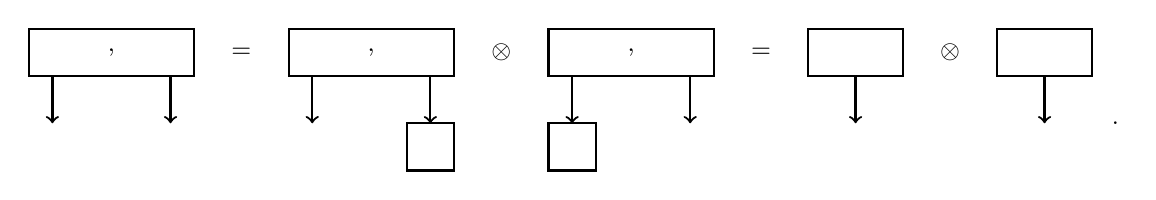
\begin{tikzpicture}[scale=0.3,thick] % , baseline = -3.5pt


\draw (0,1) rectangle (7,-1);
\node[anchor=center] (text) at (3.5,0) {\small $\probof{\exrandom,\secexrandom}$};
\draw[->] (1,-1) -- (1,-3) node[midway, left] {\tiny $\exrandom$};
\draw[->] (6,-1) -- (6,-3) node[midway, left] {\tiny $\secexrandom$};

\node[anchor=center] (text) at (9,0) {\small ${=}$};


\begin{scope}[shift={(11,0)}]

\draw (0,1) rectangle (7,-1);
\node[anchor=center] (text) at (3.5,0) {\small $\probof{\exrandom,\secexrandom}$};
\draw[->] (1,-1) -- (1,-3) node[midway, left] {\tiny $\exrandom$};
\draw[->] (6,-1) -- (6,-3) node[midway, left] {\tiny $\secexrandom$};
\draw (5,-3) rectangle (7,-5);
\node[anchor=center] (text) at (6,-4) {\small $\ones$};

\end{scope}

\node[anchor=center] (text) at (20,0) {\small $\otimes$};

\begin{scope}[shift={(22,0)}]

\draw (0,1) rectangle (7,-1);
\node[anchor=center] (text) at (3.5,0) {\small $\probof{\exrandom,\secexrandom}$};
\draw[->] (1,-1) -- (1,-3) node[midway, left] {\tiny $\exrandom$};
\draw (0,-3) rectangle (2,-5);
\node[anchor=center] (text) at (1,-4) {\small $\ones$};
\draw[->] (6,-1) -- (6,-3) node[midway, left] {\tiny $\secexrandom$};

\end{scope}

\node[anchor=center] (text) at (31,0) {\small ${=}$};

\begin{scope}[shift={(33,0)}]

\draw (0,1) rectangle (4,-1);
\node[anchor=center] (text) at (2,0) {\small $\margprobof{\exrandom}{\exrandom}$};
\draw[->] (2,-1) -- (2,-3) node[midway, left] {\tiny $\exrandom$};

\node[anchor=center] (text) at (6,0) {\small $\otimes$};

\draw (8,1) rectangle (12,-1);
\node[anchor=center] (text) at (10,0) {\small $\margprobof{\secexrandom}{\secexrandom}$};
\draw[->] (10,-1) -- (10,-3) node[midway, left] {\tiny $\secexrandom$};


\end{scope}

\node[anchor=center] (text) at (46,-3) {\small ${.}$};

\end{tikzpicture} 
	\end{center}

Independence is a very strong assumption, which is often too restrictive.
Conditional independence instead is a less demanding assumption, when certain conditional distribution variables are independent. 
This leads to tensor network decompositions with a more realistic assumption.

\begin{definition}[Conditional Independence]\label{def:condIndependence}
	Given a joint distribution of variables $\exrandom$, $\secexrandom$ and $\thirdexrandom$, we say $\exrandom$ is independent from $\secexrandom$ conditioned on $\thirdexrandom$ if for any incides $\exrandind,\secexrandind$ and $\thirdexrandind$
		\[ \condprobof{\indexedexrandom,\indexedsecexrandom}{\indexedthirdexrandom} 
		= \condprobof{\indexedexrandom}{\indexedthirdexrandom} 
		\cdot \condprobof{\indexedsecexrandom}{\indexedthirdexrandom}   \, . \]
\end{definition}

Conditional independence is a relation between conditional probabilities and is therefore equivalent to a normation equation stated next.

\begin{theorem}[Conditional Independence as a Contraction Equation]\label{the:condIndependenceProductCriterion}
	Given a distribution $\probtensor$ of variables $\exrandom$, $\secexrandom$ and $\thirdexrandom$, the variable $\exrandom$ is independent from $\secexrandom$ if and only if the contraction equation
	\begin{align*}
		 \condprobof{\exrandom,\secexrandom}{\thirdexrandom} 
		 = \sbcontractionof{
		 \condprobof{\exrandom}{\thirdexrandom} ,\condprobof{\secexrandom}{\thirdexrandom} 
		 }{\exrandom,\secexrandom,\thirdexrandom}
	\end{align*}
	holds.
\end{theorem}
\begin{proof}
	Directly by Theorem~\ref{the:conditionalContraction} used on the conditional probabilities in \defref{def:condIndependence}.
\end{proof}

We can exploit conditional independence to find tensor network decompositions of probability tensors, as we show in the next theorem.

\begin{corollary}\label{cor:secCriterionCondIndepencence}
	If and only if $\exrandom$ is independent from $\secexrandom$ conditioned on $\thirdexrandom$ the probability distribution $\probtensor$ satisfies
		\[ \probat{\exrandom, \secexrandom, \thirdexrandom} 
		= \contractionof{
			\{ \condprobof{\exrandom}{\thirdexrandom}, \condprobof{\secexrandom}{\thirdexrandom}, \margprobof{\thirdexrandom}{\thirdexrandom} \}
		}{
			\exrandom, \secexrandom, \thirdexrandom
		} \, .
		\]
\end{corollary}
\begin{proof}
	Follows from Theorem~\ref{the:condIndependenceProductCriterion} and Theorem~\ref{the:bayes}.
%	We start with the chain rule decomposition of Theorem~\ref{the:chainRule} and have
%		\[ \probat{\exrandom,\secexrandom,\thirdexrandom} = \probat{\thirdexrandom}  \cdot \condprobof{\exrandom,\secexrandom}{\thirdexrandom} \]
%	Since $\exrandom$ is independent from $\secexrandom$ conditioned on $\thirdexrandom$ we have
%		\[ \condprobof{\exrandom,\secexrandom}{\thirdexrandom}  = \condprobof{\exrandom}{\thirdexrandom}  \cdot \condprobof{\secexrandom}{\thirdexrandom}  \, . \]
%	Converse direction similar.
\end{proof}


\begin{corollary}\label{cor:conditionDropping}
	Whenever $\exrandom$ is independent of $\secexrandom$ given $\thirdexrandom$, we have
	\begin{align*}
		\condprobof{\exrandom}{\secexrandom,\thirdexrandom} = \condprobof{\exrandom}{\thirdexrandom} \, .
	\end{align*}
\end{corollary}


\begin{figure}[h]
\begin{center}
	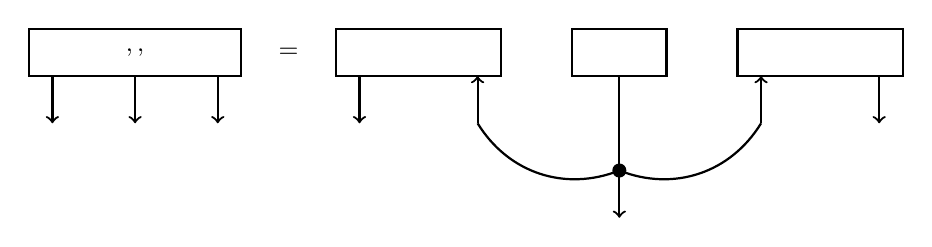
\begin{tikzpicture}[scale=0.3,thick] % , baseline = -3.5pt


\draw (-2,1) rectangle (7,-1);
\node[anchor=center] (text) at (2.5,0) {\small $\probof{\exrandom,\secexrandom,\thirdexrandom}$};
\draw[->] (-1,-1) -- (-1,-3) node[midway, left] {\tiny $\exrandom$};
\draw[->] (2.5,-1) -- (2.5,-3) node[midway, left] {\tiny $\secexrandom$};
\draw[->] (6,-1) -- (6,-3) node[midway, left] {\tiny $\thirdexrandom$};

\node[anchor=center] (text) at (9,0) {\small ${=}$};

\draw (11,1) rectangle (18,-1);
\node[anchor=center] (text) at (14.5,0) {\small $\condprobof{\exrandom}{\thirdexrandom}$};
\draw[->] (12,-1) -- (12,-3) node[midway, left] {\tiny $\exrandom$};
\draw[<-] (17,-1) -- (17,-3) node[midway, left] {\tiny $\thirdexrandom$};

\draw (21,1) rectangle (25,-1);
\node[anchor=center] (text) at (23,0) {\small $\probof{\thirdexrandom}$};
\draw (23,-1) -- (23,-3) node[midway, left] {\tiny $\thirdexrandom$};

\draw (23,-3) -- (23,-5);
\draw[fill] (23,-5) circle (0.25cm);
\draw[->] (23,-5) -- (23,-7) node[midway, left] {\tiny $\thirdexrandom$};
\draw (17,-3) to[bend right=40] (23,-5);
\draw (29,-3) to[bend right=-40] (23,-5);


\draw (28,1) rectangle (35,-1);
\node[anchor=center] (text) at (31.5,0) {\small $\condprobof{\secexrandom}{\thirdexrandom}$};
\draw[<-] (29,-1) -- (29,-3) node[midway, left] {\tiny $\thirdexrandom$};
\draw[->] (34,-1) -- (34,-3) node[midway, left] {\tiny $\secexrandom$};



\end{tikzpicture} 
\end{center}
\caption{Diagrammatic visualization of the contraction equation in Corollary~\ref{cor:secCriterionCondIndepencence}. Conditional independence of $\exrandom$ and $\secexrandom$ given $\thirdexrandom$ holds if the contraction on the right ride is equal to the probability tensor on the left side.}
\end{figure}



% More of an example?
\begin{theorem}[Markov Chain]\label{the:MarkovChain}
	Let there be a set of variables $\catvariableof{\tenumerator}$ where $\tenumeratorin$.
	When $\catvariableof{\tenumerator}$ is independent of $\catvariableof{0:{\tenumerator-2}}$ conditioned on $\catvariableof{\tenumerator-1}$ (the Markov Property), then
	\begin{align*}
		\probtensor = \contractionof{\{ \condprobof{\catvariableof{\tenumerator}}{\catvariableof{\tenumerator-1}}\, : \, \tenumeratorin \}}{
		\catvariableof{0},\ldots,\catvariableof{\tdim-1}
		} 
	\end{align*}	
%		\[ \probat{\catvariableof{0},\ldots,\catvariableof{\tdim-1}} = %\probat{\catvariableof{1}} 
%		\prod_{\tenumeratorin} \condprobof{\catvariableof{\tenumerator}}{\catvariableof{\tenumerator-1}} \, . \] 
	We depict this decomposition in Figure~\ref{fig:MC}.
\end{theorem}
\begin{proof}
	By the chain rule (Theorem~\ref{the:chainRule}) we have
	\begin{align*}
	 	\probat{\catvariableof{0},\ldots,\catvariableof{\tdim-1}}
		= \contractionof{
		\{ \condprobof{\catvariableof{\tenumerator}}{\catvariableof{0:\tenumerator}} : \tenumeratorin \}
		}{\catvariableof{[\tdim]}}
		%= \contractionof{\{\probat{\catvariableof{0}} \prod_{\tenumeratorin, \tenumerator>1} \condprobof{\catvariableof{\tenumerator}}{\catvariableof{0:\tenumerator}}\}{\catvariableof{[\tdim]}} \, . 
	\end{align*}
	Using the conditional independence of $\catvariableof{\tenumerator}$ and $\catvariableof{0:{\tenumerator-2}}$ conditioned on $\catvariableof{\tenumerator-1}$ we further have by Corollary~\ref{cor:conditionDropping}
		\[ \condprobof{\catvariableof{\tenumerator}}{\indexedcatvariableof{0:\tenumerator}}  = \condprobof{\catvariableof{\tenumerator}}{\indexedcatvariableof{\tenumerator-1}} \, .  \]
	Composing both equalities shows the claim.
\end{proof}

Here we denoted by $\catvariableof{0:\tenumerator}$ the tuple $\catvariableof{0},...,\catvariableof{\tenumerator}$.

\begin{remark}
	Let us notice that the dimensionality dropped drastically through applying the independence assumption.
	The tensor space in the naive representation of any probability distribution has
		\[ \prod_{\tenumeratorin} \catdimof{\tenumerator}\]
	coordinates, while the Markov Chain is represented by
		\[ \sum_{\tenumeratorin}  \catdimof{\tenumerator}\cdot \catdimof{\tenumerator-1} \, . \]
	Replacing exponential scaling with the number of variables to linear scaling is the advantage of tensor network decompositions.
\end{remark}

\begin{figure}[h]
\begin{center}
	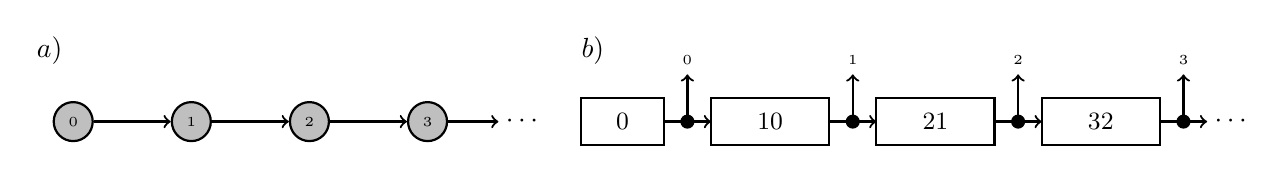
\begin{tikzpicture}[scale=0.3,thick] % , baseline = -3.5pt

\node[anchor=center] (text) at (-1,3) {${a)}$};

	\node [circle, draw, thick, fill=gray!50] (T1) at (0,0) {\tiny $\randomxof{0}$};
	\node [circle, draw, thick, fill=gray!50] (T2) at (5,0) {\tiny $\randomxof{1}$};
	\draw[->] (T1) -- (T2);
	\node [circle, draw, thick, fill=gray!50] (T3) at (10,0) {\tiny $\randomxof{2}$};
	\draw[->] (T2) -- (T3);
	\node [circle, draw, thick, fill=gray!50] (T4) at (15,0) {\tiny $\randomxof{3}$};
	\draw[->] (T3) -- (T4);
	\draw[->] (T4) -- (18,0);

	\node[anchor=center] (text) at (19,0) {$\cdots$};

	%\node [circle, draw, thick, fill=gray!50] (T4) at (17,0) {\tiny $\randomxof{\atomorder}$};
	%\draw[->] (14,0) -- (T4);	
			

\begin{scope}[shift={(25,0)}]

\node[anchor=center] (text) at (-3,3) {${b)}$};

\draw (-3.5,-1) rectangle (0, 1);
\node[anchor=center] (text) at (-1.75,0) {\small $\probof{\randomxof{0}}$};
\draw[->] (0,0) -- (2,0);
\draw[fill] (1,0) circle (0.25cm);
\draw[->] (1,0) -- (1,2) node[above] {\tiny $\catlegof{0}$};
\draw (2,-1) rectangle (7, 1);
\node[anchor=center] (text) at (4.5,0) {\small $\condprobof{\randomxof{1}}{\randomxof{0}}$};
\draw[->]  (7,0) -- (9,0);
\draw[fill] (8,0) circle (0.25cm);
\draw[->] (8,0) -- (8,2) node[above] {\tiny $\catlegof{1}$};
\draw (9,-1) rectangle (14, 1);
\node[anchor=center] (text) at (11.5,0) {\small $\condprobof{\randomxof{2}}{\randomxof{1}}$};
\draw[->]  (14,0) -- (16,0);
\draw[fill] (15,0) circle (0.25cm);
\draw[->] (15,0) -- (15,2) node[above] {\tiny $\catlegof{2}$};
\draw (16,-1) rectangle (21, 1);
\node[anchor=center] (text) at (18.5,0) {\small $\condprobof{\randomxof{3}}{\randomxof{2}}$};
\draw[->]  (21,0) -- (23,0);
\draw[fill] (22,0) circle (0.25cm);
\draw[->] (22,0) -- (22,2) node[above] {\tiny $\catlegof{3}$};
\node[anchor=center] (text) at (24,0) {$\cdots$};


\end{scope}

\end{tikzpicture} 
\end{center}
\caption{Depiction of a Markov Chain. 
	a) Dependency Graph (of the corresponding chain Graphical Model).
	b) Dual Tensor Network representing the conditional probability factors.}
\label{fig:MC}
\end{figure}





\subsection{Graphical Models}



We have already depicted conditional dependency assumptions made for Markov Chains in Figure~\ref{fig:MC} and discussed the implied decomposition of the dual tensor networks.
Graphical models provide a more general framework for conditional dependency assumptions and provide a generic approach to exploit independences in finding tensor network decompositions of $\probtensor$.


%Graphical Models are typically depicted by nodes to each variable and edges.
Following the tensor network formalism we in this section introduce graphical models based on hypergraphs.
Whether the hypergraph is directed or not distinguished between Bayesian Networks and Markov Networks.




%\begin{remark}[Further nomenclature]
%	The factors of the graphical models are tensors (since multivariate functions of discrete variables).
%	The edges are associated to each axis of the tensor and carry the variables.
%	Since each edge variable can appear in multiple factors, the Tensor Network is defined on a Hypergraph, where edges are interpreted as Hadamard contractions.
%\end{remark}



\subsubsection{Markov Networks}

While typically Markov Networks are defined on graphs, we define them here on hypergraphs to establish a direct connection to tensor networks defined on the same hypergraph.
Along that line, Markov Networks are tensor networks with non-negative tensors (see \defref{def:tensorNetwork}), which are interpreted as probability distributions after normation.

\begin{definition}[Markov Network]\label{def:markovNetwork}
	Let $\tnetof{\graph}$ be a tensor network of non-negative tensors on a hypergraph $\graph$.
	Then the Markov Network to $\tnetof{\graph}$ is the probability distribution of $\catvariableof{\node}$ defined by the tensor
		\[ \probofat{\graph}{\nodevariables} = \frac{
			\contractionof{\{\hypercoreof{\edge} : \edge \in \edges\}}{\nodevariables} 
		}{
			\contraction{\{\hypercoreof{\edge} : \edge \in \edges\}}
		} = \normationof{\tnetof{\graph}}{\nodevariables} \, . \] 
	We call the denominator
		\[\partitionfunctionof{\tnetof{\graph}} = \contraction{\{\hypercoreof{\edge} : \edge \in \edges\}} \]
	the partition function of the Markov Network.
\end{definition}

% Marginalization and Conditioning
Often, we are only interested in the distribution of a subset of variables, which are called the observable variables, and call the other variables hidden variables.
The marginalization of a Markov Network to $\tnetof{\graph}$ on the variables $\catvariableof{\secnodes}$ is
	\[
		\probofat{\graph}{\catvariableof{\secnodes}}
		= \normationof{\tnetof{\graph}}{\catvariableof{\secnodes}} \, . 
	\]
This can be derived from Theorem~\ref{the:splittingContractions}, which established an equivalence of contractions with sequences of consecutive contractions.


Further, the distribution of $\catvariableof{\secnodes}$ conditioned on $\catvariableof{\thirdnodes}$, where $\secnodes,\thirdnodes$ are disjoint subsets of $\nodes$, is
	\[
		\probtensor^{\graph}\left[ \catvariableof{\secnodes} | \catvariableof{\thirdnodes}\right] 
		= \normationofwrt{\tnetof{\graph}}{\catvariableof{\secnodes}}{\catvariableof{\thirdnodes}} \, . 
	\]

\begin{definition}[Separation of Hypergraph]
	A path in a hypergraph is a sequence of nodes $\node_{\atomenumerator}$ for $\atomenumeratorin$, such that for any $\atomenumerator\in[\atomorder-1]$ we find a hyperedge $\edge\in\edges$ such that $(\node_{\atomenumerator}, \node_{\atomenumerator+1})\subset \edge$.
	Given disjoint subsets $\nodesa$, $\nodesb$, $\nodesc$ of nodes in a hypergraph $\graph$ we say that $\nodesc$ separates $\nodesa$ and $\nodesb$ with respect to $\graph$, when any path starting at a node in $\nodesa$ and ending in a node in $\nodesb$ contains a node in $\nodesc$.
	%when removing the hyperedges which are contained in $\nodesc$ leads to a hypergraph with no path of hyperedges between a node in $\nodesa$ to a node in $\nodesb$.
\end{definition}

To characterize Markov Networks in terms of conditional independencies we need to further define the property of clique-capturing.
This property of clique-capturing established a correspondence of hyperedges with maximal cliques in an alternative graph-based definition of Markov Networks \cite{koller_probabilistic_2009}.

\begin{definition}[Clique-Capturing Hypergraph]\label{def:ccHypergraph}
	We call a hypergraph $\graph$ clique-capturing, when each subset $\secnodes\subset\nodes$ is contained in a hyperedge, if for any $a,b\in\secnodes$ there is a hyperedge $\edge\in\edges$ with $a,b\in\secnodes$.
\end{definition}

Let us now show a characterization of Markov Networks in terms of conditional independencies, which is analogous to Theorem~\ref{the:condIndBN}.

% Characterization
\begin{theorem}\label{the:condIndMN}
	Given a clique-capturing hypergraph $\graph$, the set of positive Markov Networks on the hypergraph coincides with the set of positive probability distributions, such that each for each disjoint subsets of variables $\nodesa$, $\nodesb$, $\nodesc$ we have $\catvariableof{\nodesa}$ is independent of $\catvariableof{\nodesb}$ conditioned on $\catvariableof{\nodesc}$, when $\nodesc$ separates $\nodesa$ and $\nodesb$ in the hypergraph. % called d-separation
\end{theorem}
\begin{proof}
	%=>
	%Given any Markov Network, contracting with $\onehotmapof{\atomlegindexof{\nodesc}}$ turns all hyperedges contained in $\nodesc$ to scalar factors (copying possible).
	Let there be a hypergraph $\graph$, a Markov Network $\extnet$ on $\graph$ and nodes $\nodesa,\nodesb,\nodesc \subset \nodes$, such that $\nodesc$ separates $\nodesa$ from $\nodesb$.
	Let us denote by $\nodes_0$ the nodes with paths to $\nodesa$, which do not contain a node in $\nodesc$, and by $\nodes_1$ the nodes with paths to $\nodesb$, which do not contain a node in $\nodesc$.
	Further, we denote by $\edges_0$ the hyperedges which contain a node in $\nodes_0$ and by $\edges_1$ the hyperedges which contain a node in $\nodes_1$.
	By assumption of separability, both sets $\edges_0$ and $\edges_1$ are disjoint and no node in $\nodesa$ is in a hyperedge in $\edges_1$, respectively no node in $\nodesb$ is in a hyperedge in $\edges_0$, .
	We then have
	\begin{align*}
		\normationofwrt{\extnetasset}{\catvariableof{\nodesa},\catvariableof{\nodesb}}{\indexedcatvariableof{\nodesc}} 
		= & \normationof{\extnetasset\cup\{\onehotmapof{\catindexof{\nodesc}}\}}{\catvariableof{\nodesa},\catvariableof{\nodesb}} \\
		= &  \normationof{\{\hypercoreof{\edge}\, : \, \edge\in\edges_0\}\cup\{\onehotmapof{\catindexof{\nodesc}}\}}{\catvariableof{\nodesa}}
		\otimes \normationof{\{\hypercoreof{\edge}\, : \, \edge\in\edges_1\}\cup\{\onehotmapof{\catindexof{\nodesc}}\}}{\catvariableof{\nodesb}} \, .
	\end{align*}
	By Theorem~\ref{the:condIndependenceProductCriterion}, it now follows that $\catvariableof{\nodesa}$ is independent of $\catvariableof{\nodesb}$ conditioned on $\catvariableof{\nodesc}$.
	%<= HARDER! Hammersley Clifford needed
	The converse direction, i.e. that positive distributions respecting the conditional indpendence assumptions are representable as Markov Networks, is known as the Hammersley Clifford Theorem, 
	which we will proof later in Section~\ref{sec:proofHCTheorem}.
	%for which proof we refer to Theorem~4.8 in KOLLER.
\end{proof}

% Positivity
From the proof of Theorem~\ref{the:condIndMN} Markov Networks with zero coordinates still satisfy the conditional independence assumption.
However, the reverse is not true, that is there are distributions with vanishing coordinates, which satisfy the conditional independence assumptions, but cannot be represented as a Markov Network (see Example~4.4 in \cite{koller_probabilistic_2009}).




\subsubsection{Bayesian Networks}

Compared to Markov Networks, Bayesian Networks impose further conditions on tensor networks representing a distribution.
They assume a directed hypergraph and each tensor decorating the edges to be normed according to the direction.
We will observe, that if the hypergraph is in addition acyclic, then each tensor core coincides with the conditional distribution of the underlying Markov Network.
To introduce Bayesian Networks, we extend \defref{def:hypergraphs} by introducing the property of acyclicity for hypergraphs.

%are described by directed acyclic graphs (DAG).
%The probability distribution is a Hadamard product of conditional probabilities, where each variable has a conditional probability factor conditioned on the parents variables in the graph.
%We introduce Bayesian Networks based on directed hypergraphs (see \defref{def:hypergraphs}) and define further properties.

\begin{definition}
	A directed path is a sequence $\node_{0},\ldots\node_{\secatomorder}$ such that for any $\secatomenumeratorin$ there is an hyperedge $\edge=(\incomingnodes,\outgoingnodes)\in\edges$ such that $\node_{\secatomenumerator}\in\incomingnodes$ and $\node_{\secatomenumerator+1}\in\outgoingnodes$.
	We call the hypergraph $\graph$ acyclic, if there is no path with $\secatomorder>0$ such that $\node_{0}=\node_{\secatomorder}$.
	Given a directed hypergraph $\graph=(\nodes,\edges)$ we define for any node $\nodein$ its parents by
		\[ \parentsof{\node} = \{\secnode \, : \, \exists\edge=(\incomingnodes,\outgoingnodes)\in\edges: \secnode\in\incomingnodes,\node\in\outgoingnodes \} \]
	and its non-descendants $\nondescendantsof{\node}$ as the set of nodes $\secnode$, such that there is no directed path from $\node$ to $\secnode$.
\end{definition}

Based on these additional graphical properties, we now define Bayesian Networks.

\begin{definition}[Bayesian Network]\label{def:bayesianNetwork}
	Let $\graph=(\nodes,\edges)$ be a directed acyclic hypergraph with edges of the form 
		\[ \edges = \bnedges \, . \]
	A \emph{Bayesian Network} is a decoration of each edge $(\parentsof{\node},\{\node\})$ by a conditional probability distribution
		\[ \condprobof{\catvariableof{\node}}{\catvariableof{\parentsof{\node}}} \]
	which represents the probability distribution
	\begin{align*}
		\probat{\nodevariables} = \contractionof{\{\condprobof{\catvariableof{\node}}{\catvariableof{\parentsof{\node}}} \, : \, \nodein\}}{\nodevariables} \, .
	\end{align*}
\end{definition}

%
By definition each tensor decorating a hyperedge is directed with $\catvariableof{\parentsof{\node}}$ incoming and $\catvariableof{\node}$ outgoing.
Thus, the directionality of the hypergraph is reflected in each tensor decorating a directed hyperedge.
This allows us to verify with Theorem~\ref{the:conditionalContractionPreservation} that their contraction defines a probability distribution.

% Contraction -> Now in definition!
%By definition we can represent a Bayesian network by the contraction
%\begin{align*}
%	\probtensorof{\graph} = \sbcontractionof{\{ \condprobof{\catvariableof{\node}}{\catvariableof{\parentsof{\node}}} \, : \, \node\in\nodes\}}{\nodes} \, . 
%\end{align*}

% Dual
%The dual tensor network consists of conditional probability distributions to each node $\node\in\nodes$ (see Figure~\ref{fig:BayesianFactor}b).

\begin{figure}[h]
\begin{center}
	\begin{tikzpicture}[scale=0.35,thick] % , baseline = -3.5pt

\node[anchor=center] (text) at (-1,3) {${a)}$};

	\node [circle, draw, thick, fill=gray!50] (H) at (5,0) {\tiny $\randomxof{\node}$};
	\node [circle, draw, thick, fill=gray!50] (P1) at (0,-5) {\tiny $\randomxof{0}$};	
	\node [circle, draw, thick, fill=gray!50] (P2) at (5,-5) {\tiny $\randomxof{1}$};	
	
	\node[anchor=center] (text) at (10,-5) {$\cdots$};
	\node [circle, draw, thick, fill=gray!50] (Pd) at (15,-5) {\tiny $\randomxof{\atomorder\shortminus1}$};
	
	\node [] (E) at (5,-2) {};	
	
	\draw[midarrow] (P1) -- (5,-2) ;	
	\draw[midarrow] (P2) -- (5,-2) ;	
	\draw[midarrow] (Pd) -- (5,-2) ;	
	\draw[midarrow] (5,-2) -- (H) ;	
			

\begin{scope}[shift={(25,0)}]

\node[anchor=center] (text) at (-3,3) {${b)}$};

\draw[->] (4.5,-1) -- (4.5,1) node[midway, right]{\tiny $\catvariableof{\node}$};
\draw (0,-1) rectangle (9,-4); 
\node[anchor=center] (text) at (4.5,-2.5) {\small $\condprobof{\randomxof{\node}}{\randomxof{[\atomorder]}} $};
\draw[->] (1,-6) -- (1,-4) node[midway, right]{\tiny $\catlegof{0}$};
\draw[->] (2.5,-6) -- (2.5,-4) node[midway, right]{\tiny $\catlegof{1}$};

\node[anchor=center] (text) at (5.5,-5) {$\cdots$};
	
\draw[->] (8,-6) -- (8,-4) node[midway, right]{\tiny $\catlegof{\atomorder\shortminus1}$};

\end{scope}

\end{tikzpicture} 
\end{center}
\caption{Example of a Factor of a Bayesian Network to the node $\catvariableof{\node}$ with parents $\catvariableof{0},\ldots,\catvariableof{\catorder-1}$, as subgraph $a)$ and dual tensor core $b)$.}
\label{fig:BayesianFactor}
\end{figure}


%% Marginalization and Contraction
Marginalization of a Bayesian Network are still Bayesian Networks on a graph where the edges directing to variables, which are not marginalized over, are replaced by directed edges to the children.
Conditioned Bayesian Network do not have a simple Bayesian Network representation, which is why we will treat them as Markov Networks to be introduced next.


\begin{theorem}[Independence Characterization of Bayesian Networks]\label{the:condIndBN}
	A probability distribution $\probat{\nodevariables}$ has a representation by a Bayesian Network on a directed acyclic graph $\graph=(\nodes,\edges)$, if and only if for any $\nodein$ the variables $\catvariableof{\node}$ are independent on $\nondescendantsof{\node}$ conditioned on $\parentsof{\node}$.
\end{theorem}
\begin{proof}
	We choose a topological order $\prec$ on the nodes of $\graph$, which exists since $\graph$ is acyclic.
	
	\proofrightsymbol:
	Let us assume, that the conditional independencies are satisfied and apply the chain rule with respect to that ordering to get
	\begin{align*}
		\probat{\nodevariables} =
		\contractionof{
			\condprobof{\catvariableof{\node}}{\catvariableof{\secnode} : \secnode \prec \node}
		}
		{\nodevariables} \, .
	\end{align*}
	Since $\prec$ is a topological ordering we have
		\[ \parentsof{\node} \subset \{\secnode : \secnode \prec \node\} \]
	We apply the assumed conditional independence with Corollary~\ref{cor:conditionDropping} and get
	\begin{align*}
		\probat{\nodevariables} =
		\contractionof{
			\condprobof{\catvariableof{\node}}{\catvariableof{\parentsof{\node}}}
		}
		{\nodevariables} \, .
	\end{align*}
	
	\proofleftsymbol:
	To show the converse direction, let there be a Bayesian Network $\probat{\nodevariables}$ on $\graph$.
	To show for any node $\node$, that $\catvariableof{\node}$ is independent of $\nondescendantsof{\node}$ conditioned on $\parentsof{\node}$, we reorder the tensors in the contraction
	%with respect to a set $\node_0$ 
	\begin{align*}
		& \condprobof{\catvariableof{\node},\catvariableof{\nondescendantsof{\node}}}{\indexedcatvariableof{\parentsof{\node}}} \\
		& \quad\quad = \normationofwrt{
			\{\condprobof{\catvariableof{\secnode}}{\catvariableof{\parentsof{\secnode}}} \, : \, \secnode\in\nodes\}
		}
		{\catvariableof{\node},\catvariableof{\nondescendantsof{\node}}}
		{\indexedcatvariableof{\parentsof{\node}}} \\
		& \quad\quad  = \normationof{
			\{\condprobof{\catvariableof{\secnode}}{\catvariableof{\parentsof{\secnode}}} \, : \, \secnode\in\nodes\} \cup \{\onehotmapof{\catindexof{\parentsof{\node}}}\}
		}
		{\catvariableof{\node},\catvariableof{\nondescendantsof{\node}}}\\
		&  \quad\quad = \normationof{
			\{\condprobof{\catvariableof{\secnode}}{\catvariableof{\parentsof{\secnode}}} \, : \, \secnode\in\nondescendantsof{\node}\} \cup \{\onehotmapof{\catindexof{\parentsof{\node}}}, \condprobof{\catvariableof{\node}}{\catvariableof{\parentsof{\node}}} \}
		}
		{\catvariableof{\node},\catvariableof{\nondescendantsof{\node}}} \\
		&  \quad\quad =  %\contractionof{
		 \normationof{
			\{\condprobof{\catvariableof{\secnode}}{\catvariableof{\parentsof{\secnode}}} \, : \, \secnode\in\nondescendantsof{\node}\} \cup \{\onehotmapof{\catindexof{\parentsof{\node}}}\}
		}
		{\catvariableof{\nondescendantsof{\node}}} \\
		& \quad\quad  \quad  \cdot \normationof{
			\{\condprobof{\catvariableof{\node}}{\catvariableof{\parentsof{\node}}},\onehotmapof{\catindexof{\parentsof{\node}}}\}
		}
		{\catvariableof{\node}} \\
		& \quad\quad  = \contractionof{\{
		\condprobof{\catvariableof{\nondescendantsof{\node}}}{\indexedcatvariableof{\parentsof{\node}}},
		\condprobof{\catvariableof{\node}}{\indexedcatvariableof{\parentsof{\node}}}
		\}}{\catvariableof{\node},\catvariableof{\nondescendantsof{\node}}}
		%}{\catvariableof{\node},\catvariableof{\nondescendantsof{\node}}}
	\end{align*}
	Here we have dropped in the third equation all tensors to the descendants, since their marginalization is trivial (which can be shown by a leaf-stripping argument).
	In the fourth equation we made use of the fact, that any directed path between the non-descendants and the node is through the parents of the node.
	By Theorem~\ref{the:condIndependenceProductCriterion}, it now follows that $\catvariableof{\node}$ is independent of $\nondescendantsof{\node}$ conditioned on $\parentsof{\node}$.
\end{proof}

\subsubsection{Bayesian Networks as Markov Networks}

Markov Networks are more flexible compared with Bayesian Networks, since any Bayesian Network is a Markov Network by ignoring the directionality of the hypergraph and understanding the conditional distributions as generic tensor cores.
In the next theorem we provide the conditions for the interpretation of a Markov Network as a Bayesian Network.

\begin{theorem}\label{the:MarkovToBayesian}
	Let $\tnetof{\graph}$ be a tensor network on a directed acyclic hypergraph, such that the edges are of the structure
		\[ \edges = \bnedges \]
	and each tensor $\hypercoreof{\edge}$ respects the directionality of the graph, that is each $\hypercoreof{(\parentsof{\node}, \{\node\})}$ is directed with the variables to $\parentsof{\node}$ incoming and $\node$ outgoing.
	Then $\partitionfunctionof{\tnetof{\graph}}=1$ and for each $\node\in\nodes$ we have
		\[ \bnnodecore = \normationofwrt{\tnetof{\graph}}{\catvariableof{\node}}{\catvariableof{\parentsof{\node}}} \, . \]
	In particular, $\tnetof{\graph}$ is a Bayesian Network.
\end{theorem}
\begin{proof}
	We show the claim by induction over the cardinality of $\nodes$.
	
	$\cardof{\nodes}=1$: In this case we find a unique node $\node\in\nodes$ and have $\edges=\{(\varnothing,\{\node\})\}$.
		The tensor $\hypercoreof{(\varnothing,\{\node\})}$ is then normed with no incoming variables and we thus have
			\[ \partitionfunctionof{\tnetof{\graph}} = \contraction{\tnetof{\graph}} = \contraction{\hypercoreof{(\varnothing,\{\node\})}} = 1 \]
		and
			\[ \normationof{\tnetof{\graph}}{\catvariableof{\node}} = \hypercoreof{(\varnothing,\{\node\})} \, .  \]
			
	$\cardof{\nodes}-1 \rightarrow \cardof{\nodes}$: Let there now be a directed hypergraph $\graph=(\nodes,\edges)$ and let us now assume, that the theorem holds for any tensor networks with node cardinality $\cardof{\nodes}-1$.
		Since the hypergraph is acyclic, we find a root $\node\in\nodes$ such that $\node\notin\parentsof{\secnode}$ for $\secnode\in\nodes$.
		We denote $\tnetof{\secgraph}$ the tensor network on the hypergraph $\secgraph=\{\nodes/\{\node\},\edges/\{(\parentsof{\node},\{\node\})\}\}$ with decorations inherited from $\tnetof{\graph}$.
		With Theorem~\ref{the:splittingContractions}, the directionality of $\bnnodecore$ and the induction assumption on $\tnetof{\secgraph}$ we have
		\begin{align*}
			\contraction{\tnetof{\secgraph}\cup\left\{\bnnodecore\right\}}
			 = \contraction{\tnetof{\secgraph}\cup\left\{\contractionof{\bnnodecore}{\catvariableof{\parentsof{\node}}}\right\}}
			 = \contraction{\tnetof{\secgraph}\cup\left\{\onesat{\catvariableof{\parentsof{\node}}}\right\}}
			 = 1
		\end{align*}
		and thus a trivial partition function.
		Since $\node$ does not appear in $\secgraph$, we have for any index $\catindexof{\parentsof{\nodes}}$
		\begin{align*}
			\contractionof{\tnetof{\graph}}{\catvariableof{\node},\indexedcatvariableof{\parentsof{\node}}}
			= \contractionof{\bnnodecore}{\catvariableof{\node},\indexedcatvariableof{\parentsof{\node}}}
			\cdot \contractionof{\tnetof{\secgraph}}{\indexedcatvariableof{\parentsof{\node}}}
		\end{align*}
		and thus, since $\bnnodecore$ is directed, that
		\begin{align*}
			\normationofwrt{\tnetof{\graph}}{\catvariableof{\node}}{\catvariableof{\parentsof{\node}}}
			= \bnnodecore \, .
		\end{align*}
\end{proof}

%\begin{theorem}\label{the:BayesianToMarkov}
%	Any Bayesian Network on a directed graph $\graph=(\nodes,\edges)$ is a Markov Network on a hypergraph $\secgraph=(\nodes,\secedges)$ with identical nodes and hyperedges consistent of  a hyeredge to each node with $\node$ being the only outgoing node and
%		\[  \{\tilde{\node} \, : \, (\tilde{\node},\node) \in \edges\} \,  \]
%	being the incoming nodes.
%	Each hyperedge of the Markov Network is decorated with the conditional probability distribution and the partition function is vanishing.
%\end{theorem}
%\begin{proof}
%	Each conditional probability distribution is associated with the hyperedge constructed to the representative node.
%	The contraction of all conditional probability distributions is the Bayesian Network, which corresponds with the constructed Markov Network due to the trivial partition function.
%\end{proof}

%% Bayesian Network richer
Theorem~\ref{the:MarkovToBayesian} states that Bayesian Networks are a subset of Markov Networks.
While Markov Network allow generic tensor cores, Bayesian Networks impose a local directionality condition on each tensor core by demanding it to be a conditional probability tensor.
In our diagrammatic notation, the local normation of Bayesian Networks is highlighted by the directionality of the hypergraph.
Generic Markov Networks are on undirected hypergraphs, where in general no local directionality condition is assumed.
As a consequence, tasks such as the determination of the partition functions or calculation of conditional distributions involve global contractions.


%% Conditioning
%The representation of Bayesian Networks by Markov Networks is of special interest when representing conditional distributions.
%Bayesian Networks conditioned on evidence are no longer Bayesian Networks on the same graph, but Markov Networks on a hypergraph enriched by the evidence conditioned about.


\subsubsection{Example: Hidden Markov Models}

We here extend the example of Markov Chains from Theorem \ref{the:MarkovChain} to a limited observation of the variables by observations.
Let there be the variables $\catvariableof{\tenumerator}$ (states) and $\randomeof{\tenumerator}$ (observations) with a discrete and finite time $\tenumeratorin$.

The conditional assumptions are 
\begin{itemize}
	\item $\catvariableof{\tenumerator+1}$ is independent of $\catvariableof{0:\tenumerator-1}$ and $\randomeof{0:\tenumerator}$ conditioned on $\catvariableof{\tenumerator}$
	\item $\randomeof{\tenumerator}$ is independent of all other variables conditioned on $\catvariableof{\tenumerator}$
\end{itemize}

Then the probability tensor has the decomposition 
\begin{align}
	\probat{\catvariableof{0:\tdim},\randomeof{0:\tdim}} 
	& = \prod_{\tenumeratorin}
	 \left( \condprobof{\catvariableof{\tenumerator}}{\catvariableof{0:\tenumerator-1},\randomeof{0:\tenumerator-1}} \cdot \condprobof{\randomeof{\tenumerator}}{\catvariableof{0:\tenumerator},\randomeof{0:\tenumerator-1}} \right) \\
	& = \probat{\catvariableof{0}} \cdot \condprobof{\randomeof{0}}{\catvariableof{0}} \cdot \prod_{\tenumeratorin, \tenumerator>0} 
	\left( \condprobof{\catvariableof{\tenumerator}}{\catvariableof{\tenumerator-1}} \cdot \condprobof{\randomeof{\tenumerator}}{\catvariableof{\tenumerator}} \right)
\end{align}
Here we used the Chain Rule decomposition of Theorem~\ref{the:chainRule} in the first equation and the conditional independence assumptions in the second.

We notice, that this is a Bayesian Netowork on a directed acyclic hypergraph $\graph$ consistent in nodes to each state and each observation and directed hyperedges
\begin{itemize}
	\item $(\{\catvariableof{\tenumerator}\}, \{\catvariableof{\tenumerator+1}\})$ for $\tenumerator\in[\tdim-1]$
	\item $(\{\catvariableof{\tenumerator}\}, \{\randomeof{\tenumerator}\})$ for $\tenumeratorin$
\end{itemize}


\begin{figure}[h]
\begin{center}
	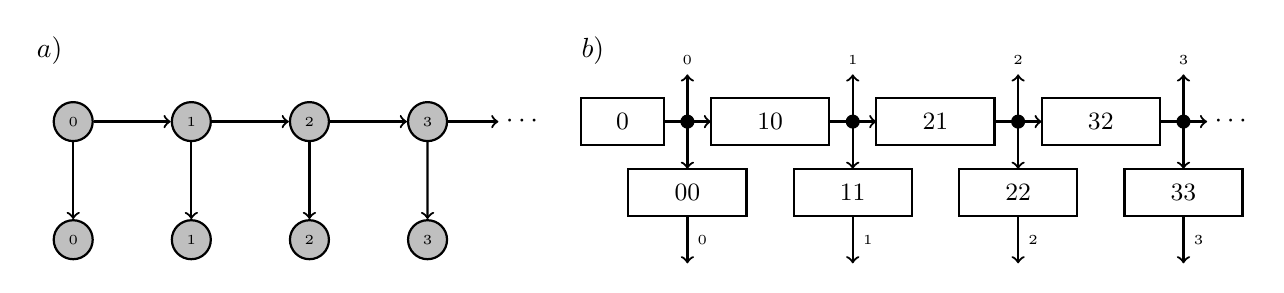
\begin{tikzpicture}[scale=0.3,thick] % , baseline = -3.5pt

\node[anchor=center] (text) at (-1,3) {${a)}$};

	\node [circle, draw, thick, fill=gray!50] (T1) at (0,0) {\tiny $\randomxof{0}$};	
	\node [circle, draw, thick, fill=gray!50] (E1) at (0,-5) {\tiny $\randomeof{0}$};
	\draw[->] (T1) -- (E1);	
	\node [circle, draw, thick, fill=gray!50] (T2) at (5,0) {\tiny $\randomxof{1}$};
	\node [circle, draw, thick, fill=gray!50] (E2) at (5,-5) {\tiny $\randomeof{1}$};
	\draw[->] (T2) -- (E2);	
	\draw[->] (T1) -- (T2);	
	\node [circle, draw, thick, fill=gray!50] (T3) at (10,0) {\tiny $\randomxof{2}$};
	\node [circle, draw, thick, fill=gray!50] (E3) at (10,-5) {\tiny $\randomeof{2}$};
	\draw[->] (T3) -- (E3);	
	\draw[->] (T2) -- (T3);
	\node [circle, draw, thick, fill=gray!50] (T4) at (15,0) {\tiny $\randomxof{3}$};
	\node [circle, draw, thick, fill=gray!50] (E4) at (15,-5) {\tiny $\randomeof{3}$};
	\draw[->] (T4) -- (E4);	
	\draw[->] (T3) -- (T4);
	\draw[->] (T4) -- (18,0);

	\node[anchor=center] (text) at (19,0) {$\cdots$};

	%\node [circle, draw, thick, fill=gray!50] (T4) at (17,0) {\tiny $\randomxof{\atomorder}$};
	%\draw[->] (14,0) -- (T4);	
			

\begin{scope}[shift={(25,0)}]

\node[anchor=center] (text) at (-3,3) {${b)}$};

\draw (-3.5,-1) rectangle (0, 1);
\node[anchor=center] (text) at (-1.75,0) {\small $\probof{\randomxof{0}}$};
\draw[->] (0,0) -- (2,0);
\draw[fill] (1,0) circle (0.25cm);
\draw[->] (1,0) -- (1,2) node[above] {\tiny ${\randomxof{0}}$};
\draw[->] (1,0) -- (1,-2);
\draw (-1.5,-2) rectangle (3.5,-4); 
\node[anchor=center] (text) at (1,-3) {\small $\condprobof{\randomeof{0}}{\randomxof{0}}$};
\draw[->] (1,-4) -- (1,-6) node[midway, right]{\tiny ${\randomeof{0}}$};

\draw (2,-1) rectangle (7, 1);
\node[anchor=center] (text) at (4.5,0) {\small $\condprobof{\randomxof{1}}{\randomxof{0}}$};
\draw[->]  (7,0) -- (9,0);
\draw[fill] (8,0) circle (0.25cm);
\draw[->] (8,0) -- (8,2) node[above] {\tiny ${\randomxof{1}}$};
\draw[->] (8,0) -- (8,-2);
\draw (5.5,-2) rectangle (10.5,-4); 
\node[anchor=center] (text) at (8,-3) {\small $\condprobof{\randomeof{1}}{\randomxof{1}}$};
\draw[->] (8,-4) -- (8,-6) node[midway, right]{\tiny ${\randomeof{1}}$};


\draw (9,-1) rectangle (14, 1);
\node[anchor=center] (text) at (11.5,0) {\small $\condprobof{\randomxof{2}}{\randomxof{1}}$};
\draw[->]  (14,0) -- (16,0);
\draw[fill] (15,0) circle (0.25cm);
\draw[->] (15,0) -- (15,2) node[above] {\tiny ${\randomxof{2}}$};
\draw[->] (15,0) -- (15,-2);
\draw (12.5,-2) rectangle (17.5,-4); 
\node[anchor=center] (text) at (15,-3) {\small $\condprobof{\randomeof{2}}{\randomxof{2}}$};
\draw[->] (15,-4) -- (15,-6) node[midway, right]{\tiny ${\randomeof{2}}$};

\draw (16,-1) rectangle (21, 1);
\node[anchor=center] (text) at (18.5,0) {\small $\condprobof{\randomxof{3}}{\randomxof{2}}$};
\draw[->]  (21,0) -- (23,0);
\draw[fill] (22,0) circle (0.25cm);
\draw[->] (22,0) -- (22,2) node[above] {\tiny ${\randomxof{3}}$};
\draw[->] (22,0) -- (22,-2);
\draw (19.5,-2) rectangle (24.5,-4); 
\node[anchor=center] (text) at (22,-3) {\small $\condprobof{\randomeof{3}}{\randomxof{3}}$};
\draw[->] (22,-4) -- (22,-6) node[midway, right]{\tiny ${\randomeof{3}}$};


\node[anchor=center] (text) at (24,0) {$\cdots$};


\end{scope}

\end{tikzpicture} 
\end{center}
\caption{Depiction of a Hidden Markov Model. 
	a) Dependency Graph (of the corresponding chain Graphical Model).
	b) Dual Tensor Network representing the conditional probability factors.}
\label{fig:HMM}
\end{figure}




\subsection{Exponential Families}\label{sec:exponentialFamilies}

% Usage of the selection encoding -> Can also make a theorem out of this
Exponential families are collections of probability distributions, where each coordinate is determined by a base measure and a set $\sstat$ of features as
	\[ \probat{\indexedshortcatvariables}  \propto \basemeasure(\catindex) \cdot \expof{\sum_{\statenumeratorin} \sstatcoordinateofat{\selindex}{\indexedshortcatvariables} \cdot \canparamat{\indexedselvariable}} \, . \]
We use the selection encoding to represent the weighted summation over the statistics, that is the tensor
	\[ \sencsstatat{\shortcatvariables,\selvariable}: \facstates \times [\statorder] \rightarrow \rr \]
with
	\[ \sencsstatat{\indexedshortcatvariables,\indexedselvariable} = \sstatcoordinateofat{\selindex}{\indexedshortcatvariables} \, . \]
We then understand $\canparam$ as a vector to the categorical variable $\selvariable$ and use Theorem~\ref{the:linCompSelEncoding} to get
	\[ \sum_{\statenumeratorin}\canparamat{\indexedselvariable}\cdot \sstatcoordinateofat{\selindex}{\shortcatvariables}
		 = \sbcontractionof{\sencsstatat{\shortcatvariables,\selvariable},\canparamat{\selvariable}}{\shortcatvariables} \, . \]

\begin{definition}
	Given a sufficient statistics 
		\[ \sstat : \facstates \rightarrow \parameterspace\]
	and a boolean base measure
		\[ \basemeasure : \facstates \rightarrow [2] \]
	with $\contraction{\basemeasure}\neq0$,  the set $\expfamily=\{\expdist \, : \, \canparam[\selvariable] \in \simpleparspace\}$ of probability distributions 
		\[ \expdistat{\shortcatvariables} = \normationof{\expof{\sbcontractionof{\sencsstat,\canparam}{\shortcatvariables},\basemeasureat{\shortcatvariables}}}{\shortcatvariables} \]
	is called the exponential family to $\sstat$.
	We further define for each member with parameters $\canparam$ the associated energy tensor
		\[ \expenergy = \sbcontractionof{\sencsstat,\canparam}{\shortcatvariables} \]
	and the cumulant function
		\[ \cumfunctionof{\canparam} = \lnof{\sbcontraction{\basemeasure,\expof{\sbcontractionof{\sencsstat,\canparam}{\shortcatvariables} }} } \, .\]
\end{definition}



% Diverging partition functions avoided here
Since we restrict the discussion to finite state spaces, the distribution $\expdist$ is well-defined for any $\canparam\in\rr^{\statorder}$.
For infinite state space there are sufficient statistics and parameters, such that the partition function $\sbcontraction{\basemeasure,\expof{\sbcontractionof{\sencsstat,\canparam}{\shortcatvariables}}}$ diverges and the normation $\expdist$ is not well-defined.
In that cases, the canonical parameters need to be chosen from a subset where the partition function is finite. 

% Restriction to boolean base measures
As before, we restrict for boolean base measures, which satisfy $\contraction{\basemeasure}\neq0$
We notice, that by positivity of the exponential function, any distribution in an exponential family $\expfamily$ is positive with respect to $\basemeasure$ (see \defref{def:positivityBaseMeasure}).
%In Chapter~\ref{cha:logicalRepresentation} these tensors will be called satisfiable propositional formulas.
In Chapter~\ref{cha:networkRepresentation} we will investigate distributions, where the base measures and the sufficient statistics share a common computation framework.



% Cumulant representation
\begin{lemma}\label{lem:energyCumulantRepresentation}
	For any member of an exponential family $\expfamily$ we have
		\[ \expdistat{\shortcatvariables} 
		= \contractionof{\expof{ \expenergy - \cumfunctionof{\canparam}\cdot \onesat{\shortcatvariables}},\basemeasureof{\shortcatvariables}}{\shortcatvariables} \, . \]
\end{lemma}
\begin{proof}
	By definition we have
	\begin{align*}
		\expdistat{\shortcatvariables} 
		&= \normationof{
		\expof{\sbcontractionof{\sencsstat,\canparam}{\shortcatvariables}},\basemeasureat{\shortcatvariables}
		}{\shortcatvariables} \\
		&= \frac{\contractionof{\expof{\sbcontractionof{\sencsstat,\canparam}{\shortcatvariables},\basemeasureat{\shortcatvariables}}}{\shortcatvariables}
			}{\contraction{\expof{\sbcontractionof{\sencsstat,\canparam	}{\shortcatvariables}},\basemeasureat{\shortcatvariables}}} \\
		&=  \frac{
		\contractionof{\expof{\expenergyat{\shortcatvariables}},\basemeasureat{\shortcatvariables}}{\shortcatvariables}
		}{
		\expof{\cumfunctionof{\canparam}}
		} \\
		& = \contractionof{\expof{ \expenergy - \cumfunctionof{\canparam}\cdot \onesat{\shortcatvariables}},\basemeasureof{\shortcatvariables}}{\shortcatvariables} \, . 
	\end{align*}
\end{proof}


% Minimal statistics

\begin{definition}[Minimal]\label{def:minimalStatistics}
	We say that a statistic $\sstat$ is minimal with respect to a boolean base measure $\basemeasure$, if there is no pair of a nonvanishing vector $\vectorat{\selvariable}$ and a scalar $\lambda\in\rr$ with
		\[ \contractionof{\sencsstatat{\shortcatvariables,\selvariable},\vectorat{\selvariable},\basemeasureat{\shortcatvariables}}{\shortcatvariables} = \lambda\cdot\basemeasureat{\shortcatvariables} \, . \]
\end{definition}




\subsubsection{Tensor Network Representation} 

We can use the relational encoding formalism to represent members of exponential families by a single contraction, as we show next.
The central insight here is a relational encoding of the sufficient statistics, which enables representation by tensor network decomposition, when the sufficient statistic is decomposable.

\begin{theorem}[Generic Representation of Exponential Families]\label{def:expFamilyTensorRep}
	Given any base measure $\basemeasure$ and a sufficient statistic $\sstat$ we enumerate for each coordinate $\selindexin$ the image $\imageof{\sstatcoordinateof{\selindex}}$ by a variable $\sstatcatof{\selindex}$ taking values in $[\cardof{\imageof{\sstatcoordinateof{\statenumerator}}}]$, given an interpretation map
		\[ \indexinterpretationof{\selindex} : 
		[\cardof{\imageof{\sstatcoordinateof{\statenumerator}}}] \rightarrow \imageof{\sstatcoordinateof{\statenumerator}} \, . \]
	
	For any parameter vector $\canparamat{\selvariable}:[\seldim]\rightarrow\rr$ we build the activation cores
		\[ \actcoreofat{\statenumerator}{\sstatcatof{\selindex}=\sstatindof{\selindex}} 
		= \expof{\canparamat{\indexedselvariable} \cdot \indexinterpretationofat{\selindex}{\sstatcatof{\selindex}} } \,   \]
	and have
		\[ \expdist = 
		\normationof{\{\basemeasure,\rencodingof{\sstat}\}\cup\{\actcoreof{\statenumerator} \, : \, \statenumeratorin\}}{\shortcatvariables} \, . 
		\]
%	where we use the vectors $\actcoreof{\statenumerator} : \imageof{\sstatcoordinateof{\statenumerator}} \rightarrow \rr $ defined for $y \in \imageof{\sstatcoordinateof{\statenumerator}}$ by
\end{theorem}
\begin{proof}
	We use an extended image of $\sstat$ by  %	which does not modify the statement of Theorem~\ref{the:tensorFunctionComposition} (since extension to cases, which are never met).
		\[ \imageof{\sstat} = \bigtimes_{\statenumeratorin} \imageof{\sstatcoordinateof{\selindex}} \, . \]
	Theorem~\ref{the:tensorFunctionComposition} implies
		\[ \expof{\sbcontractionof{\sencsstat,\canparam}{\shortcatvariables}}
		= \sbcontractionof{\rencodingof{\sstat}, \restrictionofto{\expof{\braket{\cdot, \weight}}}{\imageof{\sstat}}}{\shortcatvariables} \, . \]
	The claim follows from the equation
		\[ \restrictionoftoat{\expof{\braket{\cdot, \canparam}}}{\imageof{\sstat}}{\catvariableof{\sstatcoordinateof{0}},\ldots,\catvariableof{\sstatcoordinateof{\seldim-1}}}
		= \bigotimes_{\selindexin} \restrictionoftoat{\expof{\cdot \canparamat{\indexedselvariable}}}{\imageof{\sstatcoordinateof{\selindex}}}{\catvariableof{\sstatcoordinateof{\selindex}}}
		= \bigotimes_{\selindexin} \actcoreofat{\selindex}{\catvariableof{\sstatcoordinateof{\selindex}}} \, . \]
\end{proof}


We notice, that the relational encoding is the contraction of the relational encoding of its coordinate maps as 
	\[ \rencodingofat{\sstat}{\shortcatvariables,\sstatcatof{[\seldim]}} = \contractionof{\rencodingof{\sstatcoordinateof{0}},\ldots,\rencodingof{\sstatcoordinateof{\seldim-1}}}{\shortcatvariables,\sstatcatof{[\seldim]}} \, .  \]
We will show this property in Theorem~\ref{the:functionDecompositionBasisCP}.
One strategy to create $\rencodingof{\sstat}$ is thus the creation of the encoding of all its coordinate maps.
When the coordinate maps are sharing common components, a sparser representation can be derived through encodings of the components shared among the coordinate map encodings.


% Core types
A tensor network representation of an exponential family is thus a Markov Network consistent of two types of cores.
Computation cores are relational encodings of statistics $\rencodingof{\sstatcoordinateof{\selindex}}$.
Our intuition is that they compute the hidden variable $\catvariableof{\sstatcoordinateof{\selindex}}$, based on Basis Calculus (see Chapter~\ref{cha:basisCalculus}).
Activation cores $\actcoreof{\selindex}$ exploit the computed variable and provide, when contracted with the relational encoding, a factor 
	\[ \sbcontractionof{\rencodingof{\sstatcoordinateof{\selindex}}, \actcoreofat{\statenumerator}{\catvariableof{\statenumerator}}}{\shortcatvariables}  \]
to the Markov Network reduced to the visible coordinates $\shortcatvariables$.
The activation cores are trivial, i.e. $\actcoreofat{\selindex}{\sstatcatof{\selindex}}=\onesat{\sstatcatof{\selindex}}$, when $\canparamat{\selvariable=\selindex}=0$.
In that case 
	\[  \sbcontractionof{\rencodingof{\sstatcoordinateof{\selindex}}, \actcoreofat{\statenumerator}{\catvariableof{\statenumerator}}}{\shortcatvariables} 
	= \onesat{\shortcatvariables} \]
and both the activation core and the corresponding computation core can be dropped from the network without changing its distribution.

% Interpretation as elementary 
By \theref{def:expFamilyTensorRep} any member of an exponential family is represented by the normed contraction of a collection of unary activation cores contracted with the computation network $\rencodingofat{\sstat}{\headvariableof{[\seldim]},\shortcatvariables}$.
We understand these activation cores as a member of a simple Markov Network distributing the head variables $\headvariableof{[\seldim]}$.
This Markov Network has a graph, where the edges contain single variables, that is $\elgraph=([\seldim],\{\{\selindex\} \, : \, \selindexin\})$.
We generalize these classed of probability distributions now to generic tensor network formats representing activation cores.
%Furthermore, we define 

% Define sets of realizable distributions
\begin{definition}
	Given a statistic $\sstat$, and a hypergraph $\graph=([\seldim],\edges)$ with nodes associated to the coordinates of the statistic, we define the set of realizable distributions by
	\begin{align*}
		\realizabledistsof{\sstat,\graph} = \left\{ \normationof{\{\rencodingofat{\sstat}{\headvariableof{[\seldim]},\shortcatvariables}\} \cup \{\hypercoreofat{\edge}{\headvariableof{\edge}}\}}{\shortcatvariables}  \, : \,\hypercoreofat{\edge}{\headvariableof{\edge}} \in\bigotimes_{\selindex\in\edge}\rr^{\headdimof{\selindex}} \right\} \, .
	\end{align*}
\end{definition}

\begin{corollary}[Corollary of \theref{def:expFamilyTensorRep}]
	For any base measure $\basemeasure$ and statistic $\sstat$ we have
		\[ \expfamilyof{\sstat,\basemeasure} \subset \realizabledistsof{\sstat,\graph} \, . \]
\end{corollary}

% Proper subset
A natural question is to further ask, whether $\expfamilyof{\sstat,\basemeasure}$ is a proper subset of $\realizabledistsof{\sstat,\graph}$.
This is the case for most pairs $\sstat,\basemeasure$, since members of exponential families are positive with respect to their base measure, while in $\realizabledistsof{\sstat,\graph}$ we allow also for activation cores with vanishing coordinates, which in general do not produce positive distributions.
We will follow these intuitions in the discussion of logical reasoning, starting with \charef{cha:logicalReasoning}, and will use the formats $\realizabledistsof{\sstat,\graph}$ as hybrid formats storing probability distributions and logical knowledge bases.

%% FALSE STATEMENT? 
%We can sum multiples of the trivial tensor on the head cores without changing the distribution as we show next.
%
%\begin{theorem}
%	For any $\statenumeratorin$, the distribution is invariant under replacing $\actcoreofat{\statenumerator}{\selvariableof{\statenumerator}}$ by $\actcoreofat{\statenumerator}{\catvariableof{\statenumerator}}+\lambda\cdot \onesat{\catvariableof{\statenumerator}}$ where $\lambda\in\rr$
%\end{theorem}
%\begin{proof}
%	Follows from linearity in each head core, trivialization by trivial heads and normation.
%	
%	By linearity we have
%	\begin{align*}
%		\sbcontractionof{\rencodingof{\sstatcoordinateof{\selindex}}, (\actcoreofat{\statenumerator}{\catvariableof{\statenumerator}}+\lambda\cdot \onesat{\catvariableof{\statenumerator}})}{\shortcatvariables}
%		= 
%		\sbcontractionof{\rencodingof{\sstatcoordinateof{\selindex}}, \actcoreofat{\statenumerator}{\catvariableof{\statenumerator}}}{\shortcatvariables}
%		+\lambda\cdot  \sbcontractionof{\rencodingof{\sstatcoordinateof{\selindex}}, \onesat{\catvariableof{\statenumerator}}}{\shortcatvariables}
%		=  \sbcontractionof{\rencodingof{\sstatcoordinateof{\selindex}}, \actcoreofat{\statenumerator}{\catvariableof{\statenumerator}}}{\shortcatvariables}
%		+ \lambda \cdot \onesat{\shortcatvariables} \, .
%	\end{align*}
%\end{proof}


\begin{remark}[Comparison of relation and selection encodings]
	% Relation vs Selection encoding
	Relation encodings are in general of higher dimensions than selection encodings.
	In can thus be intractible to instantiate the probability distribution as a tensor networks, while the energy tensor can still be efficiently represented based on selection encodings.
	\red{In this case, energy-based reasoning algorithms are tractible while more direct methods are intractible.}
\end{remark}





\subsubsection{Mean Parameters}

Mean parameters are an alternative way to represent members of exponential families.

\begin{definition}\label{def:meanForwardBackward}
	Let there be an exponential family defined by a statistic $\sstat$ and a boolean base measure.
	We call the tensor
		\[ \meanparam = \sbcontractionof{\probtensor,\sencsstat}{\selvariable} \]
	the mean parameter tensor to a distribution $\probtensor$ of an exponential family.
	The set 
		\[ \genmeanset = \left\{\contractionof{\probtensor,\sencsstat,\basemeasure}{\selvariable} \, : \, 0\prec\probtensor , \, \contractionof{\probtensor,\basemeasure}{\shortcatvariables} 
		= \basemeasureat{\shortcatvariables} \right\} \, , \]
	where $\probtensorset$ denotes the set of all probability distributions,
	is called the convex polytope of realizable mean parameters.
	The map
		\[ \forwardmap :  \simpleparspace\rightarrow\simpleparspace\]
	with $\forwardmapof{\canparam} = \sbcontractionof{\expdist,\sencsstat}{\selvariable}$ is called the forward map of the exponential family and any map
		\[ \backwardmap : \imageof{\forwardmap} \rightarrow \simpleparspace\]
	with $\expdistof{(\sstat,\backwardmapof{\forwardmapof{\canparam}},\basemeasure)} = \expdist$ for any $\canparam\in\rr^{\statorder}$ a backward map.
\end{definition}


% Convex Hull Characterization Polytope
While introduced here as a property of a distribution, the mean parameters will be central to the discussion of probabilistic inference in Chapter~\ref{cha:probReasoning}.
We now provide a simple characterization of the sets of mean parameters based on slices of the selection encoding of the statistic.

\begin{theorem}\label{the:meanPolytopeConvHull}
	For any statistic $\sstat$ the polytope of mean parameters is the convex hull of the slices of $\sencsstat$ with fixed indices to $\shortcatvariables$, that is
	\begin{align*}
		\genmeanset 
		= \convhullof{\sencsstatat{\indexedshortcatvariables,\selvariable} \, : \, \shortcatindices\in\facstates, \, \basemeasureat{\indexedshortcatvariables}=1} \, . 
	\end{align*}	
\end{theorem}
\begin{proof}
	This follows from the fact, that the set of probability distributions is the convex hull of the one-hot encodings and the convex hull of mean parameters is a linear transform of that set.
\end{proof}


% Halfspace Representation
The convex polytope $\genmeanset$ can further be characterized as an intersection of half-spaces, as we state next.

\begin{theorem}\label{the:meanPolytopeHalfspaces}
	For any statistic $\sstat$ and base measure $\basemeasure$ there exists a finite collection $\halfspaceparams$ where $a_i[\selvariable]$ a vector and $b_i\in\rr$ for all $i\in[n]$ such that
	\begin{align*}
		\genmeanset
		= \left\{\meanparamat{\selvariable} \, : \, \forall_{i\in[n]} \, \contraction{\meanparamat{\selvariable},\normalvecofat{i}{\selvariable}}\leq\normalboundof{i} \right\} \, . 
	\end{align*}
\end{theorem}
\begin{proof}
	This is a standard result of combinatorical optimization, see e.g. \cite{ziegler_lectures_2013}.
\end{proof}

The determination of the the vectors $\halfspaceparams$ and is one reason for the intractability of probabilistic inference (see e.g. \cite{wainwright_graphical_2008}).



\begin{definition}\label{def:meanPolytopeFaces}
	Given a mean parameter polytope $\genmeanset$ in the half space representation of Theorem~\ref{the:meanPolytopeHalfspaces}, and any subset $\mathcal{I}\subset[n]$ we say that the set
	\begin{align*}
		\genfacesetof{\facecondset} = \left\{\meanparamat{\selvariable}\in\genmeanset \, : \, \forall_{i\in\mathcal{I}} \, \contraction{\meanparamat{\selvariable},\normalvecofat{i}{\selvariable}}\leq\normalboundof{i} \right\} 
	\end{align*}
	is the face to the constraints $\mathcal{I}$.
\end{definition}


\begin{theorem}\label{the:faceNormal}
	For any non-empty face $\genfacesetof{\facecondset}$ to a subset $\mathcal{I}\subset[n]$ there is a vector $\canparamat{\selvariable}$, which we call a normal of the face, such that
		\[ \genfacesetof{\facecondset} = \argmax_{\meanparam\in\genmeanset} \contraction{\canparamat{\selvariable},\meanparamat{\selvariable}}  \, . \]
	For any collection of positive $\lambda_i$, where $i\in\facecondset$, the vector
		\[ \canparamat{\selvariable} = \sum_{i\in\facecondset} \lambda_i\cdot\normalvecofat{i}{\selvariable}\]
	is a normal for $\genfacesetof{\facecondset}$.		
	%% UNCLEAR if this is true-> Are all possible normals in the span )
%	If $\canparamat{\selvariable}$ is a normal to a face, then for any positive scalars $\lambda[\selvariable]$ also the vector
%		\[ \seccanparam\left[\selvariable\right] = \contractionof{\canparamat{\selvariable},\labmda[\selvariable]}{\selvariable} \]
%	is a normal to the same face.
\end{theorem}
\begin{proof}
	The first claim follows trivially from the second.
	To show the second claim, let there be for $i\in\facecondset$ arbitrary positive scalars $\lambda_i$.
	We use that the face is non-empty, and thus there is a $\meanparamat{\selvariable}$ with
		\[ \contraction{\meanparamat{\selvariable},\normalvecofat{i}{\selvariable}}=\normalboundof{i} \]
	for all $i\in\facecondset$.
	Since for any $\meanparam\in\genmeanset$ 
		\[ \contraction{\meanparamat{\selvariable},\normalvecofat{i}{\selvariable}} \leq \normalboundof{i} \]
	it follows that
		\[ \max_{\meanparam\in\genmeanset} \contraction{\canparamat{\selvariable},\meanparamat{\selvariable}} 
		= \sum_{i\in\facecondset} \lambda_i \cdot \normalboundof{i} \, \, . \]
	The maximum is attained at a $\meanparamat{\selvariable}$, if and only if the equations $\contraction{\meanparamat{\selvariable},\normalvecofat{i}{\selvariable}}=\normalboundof{i}$ are satisfied for $i\in\facecondset$.
	This is equalt to $\meanparam\in\genfacesetof{\facecondset}$.
\end{proof}

% Notation
In a slide abuse of notation, we denote in this case $\genfacesetof{\canparam} = \genfacesetof{\facecondset}$.




\subsubsection{Examples}

% Minterm Exponential Family
\begin{example}[The minterm exponential family]\label{exa:mintermExpFamily}
	When taking as sufficient statistic the identity $\identityat{\shortcatvariables,\selvariableof{[\catorder]}}$, we can represent any positive distribution $\probtensor$ as a member of the exponential family, namely when choosing the canonical parameter
		\[ \canparam = \lnof{\probtensor} \, . \]
	The associated mean parameter is then, after relabeling the variables $\shortcatvariables$ by $\selvariableof{[\catorder]}$,
		\[ \meanparam = \probtensor \,  \]
	and $\meansetof{\identity,\ones}$ coincides with the set of probability tensors.
	For reasons to be explained in the Chapter~\ref{cha:logicalRepresentation} we refer to this family as the minterm exponential family.
\end{example}


% Markov Networks
Given a hypergraph with fixed node decoration, the different decorations of the hyperedges by tensors can be represented by an exponential family, as we show next.

\begin{theorem}[Exponential Representation of Markov Networks]
	For any hypergraph $\graph=(\nodes,\edges)$ we define a sufficient statistics 
		\[ \sstat = \bigtimes_{\edge\in\edges}  \sstatcoordinateof{\edge} \]
	where 
		\[ \sstatcoordinateof{\edge}(\catindexof{\nodes}) = \catindexof{\edge} \, . \]
	Given any Markov Network $\{\hypercoreof{\edge} \, : \, \edge\in\edges\}$ on $\graph$ with positive tensors $\hypercoreof{\edge}$ we define
		\[ \canparam = \bigtimes_{\edge\in\edges} \canparamof{\edge} \]
	where
		\[ \canparamof{\edge} =  \lnof{\hypercoreof{\edge}} \]
	and $\ln$ acts coordinatewise.
	Then, the Markov Network is in the member of the exponential family with trivial base measure, sufficient statistic $\sstat$ and parameters $\canparam$.
\end{theorem}
\begin{proof}
	We have for any $\catindexof{\nodes}$
	\begin{align}
	\prod_{\edge\in\edges} \hypercoreofat{\edge}{\indexedcatvariableof{\edge}}
		= \expof{\sum_{\edge\in\edges} \canparamofat{\edge}{\indexedcatvariableof{\edge}}}
		= \expof{\sum_{\edge\in\edges} \sbcontraction{\canparamofat{\edge}{\catvariableof{\edge}},\sstatcoordinateof{\edge}(\catindexof{\nodes})}}  \, .
	\end{align}
	Using that
		\[ \contractionof{\sstat,\canparam}{\nodevariables} = \sum_{\edge\in\edges} \contractionof{\sstatcoordinateof{\edge},\canparamof{\edge}}{\nodevariables} \]
	we get
	\begin{align}
		\contractionof{\{\hypercoreof{\edge}: \edge\in\edges\}}{\nodevariables} = \expof{\contractionof{\canparam,\sstat}{\nodevariables}} \, .
	\end{align}
	This implies 
	\begin{align}
		\normationof{\{\hypercoreof{\edge}: \edge\in\edges\}}{\nodevariables} = \normationof{\expof{\contractionof{\canparam,\sstat}{\nodevariables}}}{\nodevariables} \, .
	\end{align}
\end{proof}


% Mean parameters
The mean parameter of the Markov Network exponential family is the cartesian product of the marginals $\meanparamofat{\edge}{\catvariableof{\edge}}$ are often refered to as beliefs in the literature.
\red{They are outer bounded by local consistency polytope, which leads to the motivation of message passing algorithms!}

\subsection{Empirical Distributions}\label{sec:empDistribution}

Let us now apply the formalism of probability distributions in tensor network representations to encode data.
\begin{definition}\label{def:dataMap}
	Given a dataset $\dataset$ of samples of the factored system we define the sample selector map
		\[ \datamap : [\datanum] \rightarrow \facstates \]
	elementwise by 
		\[ \datamapof{\dataindex} = (\catindicesof{\dataindex}) \, . \]
	%% Empirical Distribution
	The empirical distribution to the sample selector map $\datamap$ is the probability distribution
	\begin{align*}
		\empdistributionat{\shortcatvariables}
		\coloneqq \sbnormationof{\datacore}{\shortcatvariables} \, ,
	\end{align*}
	where by $\datacore$ we denote the relational encoding (see \defref{def:functionRepresentation}) of the sample selector map, and the distributed variables $\shortcatvariables$ are the head variables of the relational encoding.
\end{definition}

% Sample Selector map (former data tensor)
The relational encoding of the sample selector map is the sum 
	\[ \datacoreat{\datvariable,\shortcatvariables} 
	= \sum_{\dataindexin} \onehotmapofat{\dataindex}{\datvariable} \otimes \onehotmapofat{\catindicesof{\dataindex}}{\shortcatvariables} \, . \]
% Interpretation of the empirical distribution
Each coordinate $\shortcatindices$ of the empirical distribution can be calculated by
\begin{align*}
	\empdistributionat{\indexedshortcatvariables} 
	= \frac{1}{\sbcontraction{\datacore}} \left( \sum_{\dataindexin} \onehotmapofat{\catindicesof{\dataindex}}{\indexedshortcatvariables}  \right) 
	= \frac{\cardof{\dataindexin \, : \, (\catindicesof{\dataindex}) = (\catindices)}}{\cardof{\dataindexin}}
\end{align*}
and is thus interpreted as the frequency of the corresponding world in the data.

%% Basic CP Decomposition 
The relational encoding of the sample selector map is a sum of one-hot encodings of the data indices and the corresponding sample states.
Such sums of basis tensors will be further investigated in Section~\ref{sec:basisCP} as basis CP decompositions.
We now exploit this structure to find efficient tensor network decompositions (see Figure~\ref{fig:DataDecomposition}) based on matrices encoding its variables.


\begin{figure}[h]
\begin{center}
	\begin{tikzpicture}[scale=0.35, thick] % , baseline = -3.5pt


\begin{scope}[shift={(-15,2)}]

\node[anchor=center] (text) at (-1,3) {${a)}$};


\node [circle, draw, thick, fill=gray!50, minimum size = \nodeminsize] (T1) at (0,0) {\tiny $\randomxof{0}$};	
\node [circle, draw, thick, fill=gray!50, minimum size = \nodeminsize] (T2) at (3,0) {\tiny $\randomxof{1}$};	
\node[anchor=center] (text) at (6,0) {\small $\cdots$};
\node [circle, draw, thick, fill=gray!50,minimum size = \nodeminsize] (T3) at (9,0) {};
\node[anchor=center] (text) at (9,0) {\tiny $\randomxof{\atomorder-1}$};	

\node [circle, draw, thick, fill=gray!50, minimum size = \nodeminsize] (C) at (4.5,-5) {};
\node[anchor=center] (text) at (4.5,-5){ \tiny $\datavariable$};	

\draw[->] (C) -- (T1) node [midway,left] {$\edgeof{0}$};
\draw[->] (C) -- (T2) node [midway,right] {$\edgeof{1}$};
\draw[->] (C) -- (T3) node [midway,right] {$\edgeof{\catorder-1}$};

\end{scope}

\node[anchor=center] (text) at (-1,5) {${b)}$};




\drawatomindices{0}{2}
\draw (-1,1) rectangle (5,-1);
\node[anchor=center] (text) at (2,0) {$\datacore$};
\draw[<-] (2,-1) -- (2,-3) node[midway, right] {\tiny $\datavariable$};

\node[anchor=center] (text) at (7,0) {${=}$};


\begin{scope}[shift={(10,2)}]

\newcommand{\conposseldec}{4.5,-5.5}

\draw[fill] (\conposseldec) circle (0.25cm);
\draw[<-] (\conposseldec) -- (4.5,-7.5) node[midway, right] {\tiny $\datavariable$};
%\draw[dashed] (3.5,-7.5) rectangle (5.5, -9.5);
%\node[anchor=center] (text) at (4.5,-8.5) {\small $\frac{1}{\datanum} \ones$};

\draw[<-] (0,1) -- (0,-1) node[midway,left] {\tiny $\catvariableof{0}$};
\draw (-1,-1) rectangle (1, -3);
\node[anchor=center] (text) at (0,-2) {\small $\datacoreof{0}$};
\draw[<-] (0,-3) to[bend right=20] (\conposseldec);


\draw[<-] (3,1) -- (3,-1) node[midway,left] {\tiny $\catvariableof{1}$};
\draw (2,-1) rectangle (4, -3);
\node[anchor=center] (text) at (3,-2) {\small $\datacoreof{1}$};
\draw[<-] (3,-3) to[bend right=20]  (\conposseldec);

\node[anchor=center] (text) at (6,-2) {$\cdots$};

\draw[<-] (9,1) -- (9,-1) node[midway,left] {\tiny $\catvariableof{\atomorder-1}$};
\draw (7.75,-1) rectangle (10.25, -3);
\node[anchor=center] (text) at (9,-2) {\small $\datacoreof{\atomorder-1}$};
\draw[<-] (9,-3) to[bend left=20]  (\conposseldec);




\end{scope}

		


\end{tikzpicture}
\end{center}
\caption{
	Representation of a dataset $\dataset$.
	a) Interpretation as a data selection variable $\datvariable$ selecting states for the variables $\shortcatvariables$.
	b) Corresponding decomposition of the relational encoding $\datacore$ into a tensor network in the basis $\cpformat$ Format (see Section~\ref{sec:basisCP}), where $\hypercoreof{\edgeof{\atomenumerator}}=\datacoreof{\atomenumerator}$.
	%Without the contraction with the dashed $\frac{1}{\datanum}\onesat{\datvariable}$ core, the datacore encodes the distribution conditioned on a datapoint. 
}
\label{fig:DataDecomposition}
\end{figure}


\begin{theorem}\label{the:empCPRep}
	Given a data map $\datamap: [\datanum] \rightarrow \facstates$ we define for $\catenumeratorin$ its coordinate maps
		\[ \datamap_{\catenumerator} : [\datanum] \rightarrow [\catdimof{\catenumerator}] \]
	by
		\[  \datamap_{\catenumerator}(\dataindex) = \catindexof{\catenumerator}^\dataindex \, .  \]
	We then have
	\begin{align*}
		\rencodingofat{\datamap}{\datvariable,\shortcatvariables}  
		= \contractionof{
		\{\rencodingofat{\datamap^{\atomenumerator}}{\datvariable,\catvariableof{\atomenumerator}} : \atomenumeratorin \} 
		}{\datvariable,\shortcatvariables} 
	\end{align*}
	and
	\begin{align*}
	\empdistributionat{\shortcatvariables}
	= \sbcontractionof{\datacoreat{\datvariable,\shortcatvariables}, \frac{1}{\datanum}\onesat{\datvariable}}{\shortcatvariables} 
	= \sbcontractionof{\datacoreofat{0}{\datvariable,\catvariableof{0}},\ldots,\datacoreofat{\catorder-1}{\catvariableof{\catorder-1}}, \frac{1}{\datanum}\onesat{\datvariable}}{\shortcatvariables} \, . 
	\end{align*}
	In a contraction diagram this reads
	\begin{center}
		\begin{tikzpicture}[scale=0.35, thick] % , baseline = -3.5pt






\drawatomindices{0}{2}
\draw (-1,1) rectangle (5,-1);
\node[anchor=center] (text) at (2,0) {$\empdistribution$};


\node[anchor=center] (text) at (7,0) {${=}$};

\node[anchor=center] (text) at (22,-1) {${\cdot}$};

\begin{scope}[shift={(10,2)}]

\newcommand{\conposseldec}{4.5,-5.5}

\draw[fill] (\conposseldec) circle (0.25cm);
\draw[<-] (\conposseldec) -- (4.5,-7.5) node[midway, right] {\tiny $\datavariable$};
\draw (3.5,-7.5) rectangle (5.5, -9.5);
\node[anchor=center] (text) at (4.5,-8.5) {\small $\frac{1}{\datanum} \ones$};

\draw[<-] (0,1) -- (0,-1) node[midway,left] {\tiny $\catvariableof{0}$};
\draw (-1,-1) rectangle (1, -3);
\node[anchor=center] (text) at (0,-2) {\small $\datacoreof{0}$};
\draw[<-] (0,-3) to[bend right=20] (\conposseldec);


\draw[<-] (3,1) -- (3,-1) node[midway,left] {\tiny $\catvariableof{1}$};
\draw (2,-1) rectangle (4, -3);
\node[anchor=center] (text) at (3,-2) {\small $\datacoreof{1}$};
\draw[<-] (3,-3) to[bend right=20]  (\conposseldec);

\node[anchor=center] (text) at (6,-2) {$\cdots$};

\draw[<-] (9,1) -- (9,-1) node[midway,left] {\tiny $\catvariableof{\atomorder-1}$};
\draw (7.75,-1) rectangle (10.25, -3);
\node[anchor=center] (text) at (9,-2) {\small $\datacoreof{\atomorder-1}$};
\draw[<-] (9,-3) to[bend left=20]  (\conposseldec);



\end{scope}

		


\end{tikzpicture}
	\end{center}
\end{theorem}
\begin{proof}
	The first claim is a special case of Theorem~\ref{the:functionDecompositionBasisCP}, to be shown in Chapter~\ref{cha:tensorEncodings}.
	To show the second claim we notice
		\[ \sbcontraction{\datacore} = \sum_{\datindexin} \sbcontraction{\rencodingofat{\datamap}{\datvariable=\datindex,\shortcatvariables}} = \datanum \,  . \]
	With the first claim it now follows that
	\begin{align*}
		\empdistributionat{\shortcatvariables}
		 = \sbnormationof{\datacore}{\shortcatvariables}
		 = \frac{\sbcontractionof{\datacore}{\shortcatvariables}}{\sbcontraction{\datacore}} 
		 =  \contractionof{
		\{\rencodingofat{\datamap^{\atomenumerator}}{\datvariable,\catvariableof{\atomenumerator}} : \atomenumeratorin \} \cup \{ \frac{1}{\datanum} \onesat{\datvariable} \}
		}{\datvariable,\shortcatvariables}  \, . 
	\end{align*}
\end{proof}


The cores $\datacoreof{\atomenumerator}$ are matrices storing the value of the categorical variable $\catvariableof{\atomenumerator}$ in the sample world indexed by $\dataindex$.

% Interpretation
From the proof of Theorem~\ref{the:empCPRep} we notice that the scalar $\frac{1}{\datanum}$ could be assigned with any core in a representation of $\empdistribution$, and the core $\onesat{\datvariable}$ is thus redundant in the contraction representation.
However, creating the core $\frac{1}{\datanum}\onesat{\datvariable}$ provides us with a simple interpretation of the empirical distribution.
We can understand $\frac{1}{\datanum}\onesat{\datvariable}$ as the uniform probability distribution over the samples, which is by the map $\datamap$ forwarded to a distribution over $\facstates$.
The one-hot encoding of each sample is itself a probability distribution, which is understood as conditioned on the respective state of the sample selection variable $\datvariable$.
The conditional distribution $\datacore$ therefore forwards the uniform distribution of the samples to a distribution of the variables $\shortcatvariables$.
In the perspective of a Bayesian Network (see Figure~\ref{fig:DataDecomposition}, the variable $\datvariable$ served as single parent for each categorical variable $\catvariableof{\catenumerator}$.


%%% Inductive vs Deductive perspective
%Each evidence is a probability distribution
%\begin{itemize}
%	\item Inductive Reasoning: When we interpret evidence as a datapoint, they are typically a basis tensor specifying precisely a world.
%	\item Deductive Reasoning: Evidence is a partial observation of the world, typically basis vectors at each variable, but leaving some unspecified ($\ones$).
%	We then interpret the evidence as being a uniform distribution over the worlds not contradicting with the evidence.
%\end{itemize}


\subsection{Discussion and Outlook}

\begin{remark}[Alternative definitions of graphical models]
	In the literature, tensor networks are often called dual to the hypergraphs defining graphical models (see e.g. \cite{robeva_duality_2019}).
	The duality becomes clear, when one interpretes the tensors as cores and their common variables as edges.
	We in this work avoid this ambiguity by directly defining tensor networks as decoration of hyperedges by tensors.
	
	Often, the tensors decorating hyperedges are called factors and their logarithm features \cite{koller_probabilistic_2009}.
	
	Further, we directly use hypergraphs instead of the more canonical association of factors with cliques of a graph.
	This avoids the discussion of non-maximal cliques as decorated with trivial tensors.
	Such hypergraphs follow the same line of though compared with factor graphs, which are bipartite graphs with nodes either corresponding with single variables or with a collection of them affected by a factor.
\end{remark}







